\documentclass{sadhana}

%% packages suggested by the Sadhana sample file
\usepackage{graphicx,amsmath,bm}
%% additional standard packages
\usepackage{booktabs,multirow,array,amssymb}
\usepackage[hidelinks]{hyperref}

\newcommand{\algname}{ArchTree}
\newcommand{\rmg}{ArchTree-RMG}
%% S-numbering of every object in the supplement
\renewcommand{\thesection}{S\arabic{section}}
\renewcommand{\thetable}{S\arabic{table}}
\renewcommand{\thefigure}{S\arabic{figure}}
\renewcommand{\theequation}{S\arabic{equation}}
\setcounter{topnumber}{3}\setcounter{dbltopnumber}{3}\setcounter{totalnumber}{4}
\renewcommand{\topfraction}{0.92}\renewcommand{\dbltopfraction}{0.92}\renewcommand{\textfraction}{0.06}\renewcommand{\floatpagefraction}{0.8}\renewcommand{\dblfloatpagefraction}{0.8}
\setlength{\emergencystretch}{1.5em}
\newcommand{\tn}[1]{\par\vspace{2pt}{\scriptsize #1\par}}
\newcommand{\main}[1]{main paper, #1}

\begin{document}

\title{Supplementary material for: Neural architecture search via trie-based deduplication and zero-cost proxies, with hardware-aware coverage: An empirical study of LLM-guided warm-start}

\author{Imaad Hajwane\textsuperscript{1,*}\and Jayshree Ghorpade-Aher\textsuperscript{1}}
\affilOne{\textsuperscript{1}Department of Computer Engineering and Technology, School of Computer Science and Engineering, Dr. Vishwanath Karad MIT World Peace University, Pune 411038, India\\ e-mail: iamimaad2kk3@gmail.com; jayshree.aher@mitwpu.edu.in}

\twocolumn[{
\maketitle
\vspace*{-4pt}
\noindent\textbf{Contents.} This document gives the material that supports the main paper but did not fit within its page limit: the detailed search loop and its settings (section~\ref{s:loop}); the status of the formal statements and the landscape measurements behind them (section~\ref{s:theory}); full proxy and cost tables (section~\ref{s:proxy}); every per-cell result at a fixed proposal budget (section~\ref{s:fixed}) and at equal GPU-hours (section~\ref{s:egh}); all rank-based statistics (section~\ref{s:stats}); the proposer $\times$ gate grid (section~\ref{s:grid}); the ablations and sensitivity studies (section~\ref{s:abl}); NAS-Bench-101 (section~\ref{s:nb101}); the LLM studies (section~\ref{s:llm}); hardware-aware search (section~\ref{s:hw}); and the seeds, reproducibility checks and data checksums (section~\ref{s:repro}). Supplementary objects are numbered S1, S2, \dots\ and always named (Table S5, Figure S3); numbers without the prefix refer to the main paper, and S1--S4 written alone denote the development stages of the main paper. Every value in the tables and figures is computed by two scripts (\texttt{make\_supp\_tables.py}, \texttt{make\_supp\_figures.py}) directly from the result files in the public repository (https://github.com/Imaadhajwane/Arch-Tree-LLM); nothing is typed by hand. Test accuracies are in \%, differences in percentage points (pt), and all results use 12 seeds unless stated otherwise. A difference is called a win or a loss only if it is significant after Holm correction within its family (paired two-sided Wilcoxon test, $p_{\mathrm{Holm}}<0.05$); W/T/L denotes wins/ties/losses of \rmg{} (or of \algname{} where the gate is held fixed).
\vspace{10pt}
}]

\corres
\volnum{}
\issuenum{}
\monthyear{}
\pgfirst{}
\pglast{}
\doinum{}
\articleType{}

\markboth{Imaad Hajwane and Jayshree Ghorpade-Aher}{Supplementary material: trie deduplication and zero-cost gating}
\onecolumn

%% =====================================================================
\section{Naming, search loop and settings}\label{s:loop}

Table~\ref{t:names} maps the identifiers used in the result files to the names used in the paper, so that every number can be traced back to its source. Figure~\ref{f:loop} expands the five-step summary of the search loop (Figure~2) into its seven operations, and Table~\ref{t:settings} lists every setting that the code actually reads; keys present in the configuration file but not read by any script are not reported.

\begin{table}[tbp]
\caption{Identifiers in the result files and the corresponding names in the paper.}\label{t:names}
\centering\footnotesize
\begin{tabular}{@{}>{\raggedright\arraybackslash}p{0.27\textwidth}>{\raggedright\arraybackslash}p{0.22\textwidth}>{\raggedright\arraybackslash}p{0.45\textwidth}@{}}
\toprule
Identifier(s) in the CSV files & Name in the paper & Description\\
\midrule
\texttt{archtree\_v1}, \texttt{archtree\_trie\_only} & S1, \algname-base & trie, raw-reward UCB ($C=\sqrt2$, mean backup), no gate\\
\texttt{archtree\_zc}, \texttt{archtree\_phase2} & S2 & S1 with the supervised gate (1,500 labelled architectures)\\
\texttt{archtree} + gate \texttt{none} & S3, \algname-RM & rank-normalised UCB ($C=0.3$, max backup) with mutation, no gate\\
\texttt{archtree\_llm}, \texttt{archtree\_headline}, \texttt{archtree\_v2}, \texttt{archtree\_zc\_unsup}, \texttt{v2} & S4, \rmg & \algname-RM with the label-free gate; LLM prior off ($\alpha=0$)\\
\texttt{archtree\_llm\_hw} & \algname-HW & rank UCB with max backup, no gate, no mutation, latency-penalised reward\\
\texttt{costpen}, \texttt{costpen025} & cost penalty $\lambda=1$, $0.25$ & gate score $S_\lambda=z(P)-\lambda z(D)$, $D=\log(1+\#\text{params})$\\
\texttt{zc}, \texttt{zc\_unsup}, \texttt{params} & supervised, label-free, \#params gate & gate applied to any proposer\\
\texttt{flat\_ucb\_none}, \texttt{flat\_ucb\_set} & flat UCB (A7) & per-position UCB without / with a set-based deduplication\\
\texttt{v1}, \texttt{rank}, \texttt{mut\_only}, \texttt{re} (design) & design-ablation arms & base + gate; rank reward only; mutation only; RE with the same gate\\
\texttt{llm\_off}, \texttt{llm\_on}, \texttt{llm\_described}, \texttt{size\_prior} & LLM-study arms & $\alpha=0$; LLM prior; operations described without names; FLOP-size prior without an LLM\\
\bottomrule
\end{tabular}
\end{table}

\begin{figure}[tbp]
\centering
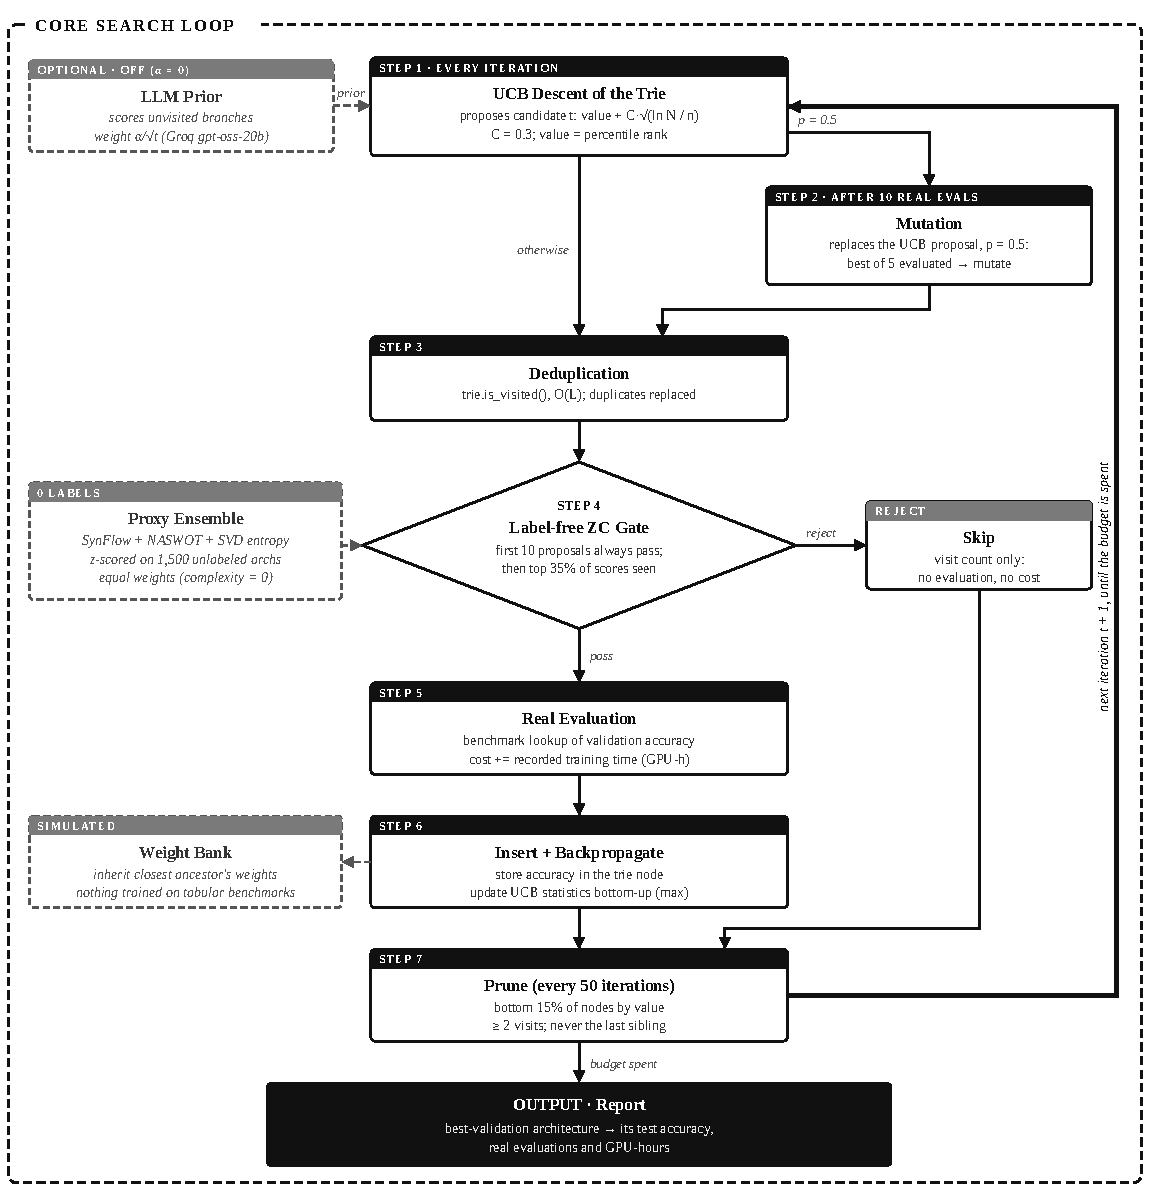
\includegraphics[width=0.74\textwidth]{figs/figS1_loop.pdf}
\caption{The search loop of \rmg{} in detail. Each iteration descends the trie by rank-normalised UCB (step 1) or, with probability 0.5 after ten real evaluations, replaces the proposal by a tournament mutation (step 2); the trie rejects architectures already seen (step 3); the label-free gate admits every proposal until ten real evaluations have been made and then only those in the top 35\% of the scores observed so far (step 4); admitted architectures receive a real evaluation (step 5), are inserted with their accuracy, which is backed up along the path (step 6), and every 50 iterations the lowest 15\% of nodes by backed-up value are pruned (step 7). Dashed boxes are optional or zero-cost components: the LLM prior (off in the headline system), the proxy ensemble and the weight bank, which has no effect on tabular benchmarks.}
\label{f:loop}
\end{figure}

\begin{table}[tbp]
\caption{Settings of the search as read by the code (identical in every reported run unless an experiment varies them).}\label{t:settings}
\centering\footnotesize
\begin{tabular}{@{}llll@{}}
\toprule
Component & Setting & Value & Varied in\\
\midrule
UCB & exploration constant $C$ & 0.3 (S1: $\sqrt2$) & Table~\ref{t:ucb}\\
 & reward / backup & percentile rank / max (S1--S2: raw / mean) & Table~\ref{t:design}\\
Mutation & share of proposals, start & 0.5, after 10 real evaluations & Table~\ref{t:design}\\
 & tournament size & 5 evaluated architectures & --\\
Gate & warm-up / pass rate & first 10 real evaluations / top 35\% of scores seen & Figure~4\\
 & proxies, calibration & $E$, $S$, $T$; z-scores from 1,500 unlabelled architectures & Table~\ref{t:subsets}\\
 & proxy network & 32 channels, fixed initialisation seed 1234 & --\\
 & NASWOT batches & 3 batches of 256 CIFAR-10 images & --\\
Pruning & period / share / eligibility & every 50 iterations / 15\% / $\geq 2$ visits, by value & Table~\ref{t:a5}\\
LLM prior & $\alpha$, decay, floor & 0 (headline), $\alpha/\sqrt{t'}$, stop below 0.02 & Table~\ref{t:alpha}\\
 & model, temperature, max tokens & \texttt{openai/gpt-oss-20b}, 0.1, 300 & Table~\ref{t:llmsize}\\
 & calls per run & at most 60 & --\\
Hardware & latency penalty & $0.05\cdot\min(\mathrm{lat}/50\,\mathrm{ms},1)$ on the 0--1 reward & --\\
Protocol & search / report metric & 200-epoch validation / test accuracy & --\\
 & budgets & NB201: 25--200 proposals; NB101: 50--400 & --\\
\bottomrule
\end{tabular}
\end{table}

%% =====================================================================
\section{Formal statements and the landscape behind them}\label{s:theory}

The early design documents of the project made seven formal claims (T1--T7). Table~\ref{t:theory} records what can and cannot be said for each, so that no statement in the main paper rests on an unproven result. The main paper uses T1, T2 and T5 only as properties of the design and makes no regret claim.

\begin{table}[tbp]
\caption{Status of the formal statements.}\label{t:theory}
\centering\footnotesize
\begin{tabular}{@{}l>{\raggedright\arraybackslash}p{0.30\textwidth}l>{\raggedright\arraybackslash}p{0.43\textwidth}@{}}
\toprule
Id & Statement & Status & Comment\\
\midrule
T1 & trie insertion and look-up cost $O(L)$ & holds & one step per token; $L=6$ on NB201\\
T2 & no architecture is evaluated twice & holds by construction & visited leaves are redirected to an unvisited one; confirmed empirically (0 repeats in every \algname{} run, Table~\ref{t:dups})\\
T3 & sub-linear regret of UCB over the trie & informal only & relies on prefix locality (Table~\ref{t:landscape}); the max backup and rank reward depart from the settings of the UCT and HOO analyses \cite{kocsis2006,coquelin2007,bubeck2011}; treated as motivation, not as a guarantee\\
T4 & pruning never removes the optimum & false as stated & value-based pruning is a heuristic without confidence bounds; its effect is measured instead (Table~\ref{t:a5})\\
T5 & weight inheritance is consistent & holds & no measurable effect on tabular benchmarks, where nothing is trained (A3: identical runs, Table~\ref{t:toggles})\\
T6 & the LLM prior preserves the regret behaviour & near-trivial & the prior only reorders never-visited siblings; a zero-information prior reproduces $\alpha=0$ exactly (24/24 seeds)\\
T7 & hypervolume ratio equals 1 iff the whole Pareto front is found & definitional & used only as a descriptive metric\\
\bottomrule
\end{tabular}
\end{table}

\textit{Prefix locality.} Statement T3 needs architectures that share a prefix to have similar accuracy. Table~\ref{t:landscape} and Figure~\ref{f:landscape} measure this on the whole NAS-Bench-201 space. The first three edges explain little of the variance ($\eta^2\le 0.13$, 0.19 and 0.24 on the three datasets), and the spread within a three-token prefix (7.8--10.8\,pt) is almost that of the whole space. Locality appears only at depth four ($\eta^2$ = 0.47--0.59). Statistics collected near the root of the trie therefore carry little information about unvisited leaves, which is consistent with the finding that the tree adds nothing beyond deduplication (section~\ref{s:abl}). The number of depth-$k$ cells that contain a leaf within 1\,pt of the optimum grows as $5^{\gamma k}$ with $\gamma$ = 0.54, 0.30 and 0.32; CIFAR-10 has many near-optimal architectures (376 leaves within 1\,pt), which explains why all good methods saturate on it.

\begin{table}[tbp]
\caption{Prefix locality of NAS-Bench-201 (all 15,625 architectures, validation accuracy): variance explained by the first $k$ tokens ($\eta^2$), mean within-prefix standard deviation, and number of prefixes $N_k(\varepsilon)$ that contain an architecture within $\varepsilon$\,pt of the best; $\gamma$ is the fitted growth exponent $N_k\propto5^{\gamma k}$.}\label{t:landscape}
\centering\footnotesize
\begin{tabular}{@{}lrrrrrrrrr@{}}
\toprule
Dataset & $k$ & prefixes & $\eta^2$ & within s.d. & $N_k(0.25)$ & $N_k(0.5)$ & $N_k(1)$ & $N_k(2)$ & $N_k(4)$\\
\midrule
CIFAR-10 & 1 & 5 & 0.063 & 11.55 & 3 & 4 & 5 & 5 & 5\\
 & 2 & 25 & 0.118 & 11.01 & 5 & 9 & 13 & 21 & 25\\
 & 3 & 125 & 0.131 & 10.77 & 10 & 22 & 46 & 90 & 125\\
 & 4 & 625 & 0.471 & 6.01 & 10 & 23 & 76 & 269 & 546\\
 & 5 & 3,125 & 0.577 & 4.10 & 17 & 51 & 212 & 811 & 2308\\
 & 6 & 15,625 & 1.000 & 0.00 & 21 & 70 & 376 & 1660 & 7190\\
 & \multicolumn{4}{r}{fitted $\gamma$} & 0.24 & 0.35 & 0.54 & 0.73 & 0.91\\
\midrule
CIFAR-100 & 1 & 5 & 0.097 & 10.98 & 1 & 1 & 2 & 2 & 5\\
 & 2 & 25 & 0.165 & 10.42 & 1 & 2 & 4 & 8 & 20\\
 & 3 & 125 & 0.188 & 10.15 & 1 & 4 & 12 & 21 & 79\\
 & 4 & 625 & 0.495 & 6.53 & 1 & 4 & 12 & 23 & 250\\
 & 5 & 3,125 & 0.612 & 4.76 & 2 & 5 & 19 & 55 & 707\\
 & 6 & 15,625 & 1.000 & 0.00 & 2 & 5 & 22 & 84 & 1319\\
 & \multicolumn{4}{r}{fitted $\gamma$} & 0.10 & 0.19 & 0.30 & 0.44 & 0.71\\
\midrule
ImageNet16-120 & 1 & 5 & 0.142 & 8.38 & 2 & 2 & 3 & 5 & 5\\
 & 2 & 25 & 0.219 & 7.98 & 3 & 6 & 9 & 16 & 20\\
 & 3 & 125 & 0.242 & 7.83 & 4 & 7 & 17 & 45 & 86\\
 & 4 & 625 & 0.587 & 5.17 & 5 & 9 & 22 & 88 & 261\\
 & 5 & 3,125 & 0.705 & 3.98 & 6 & 13 & 36 & 197 & 794\\
 & 6 & 15,625 & 1.000 & 0.00 & 6 & 17 & 46 & 278 & 1601\\
 & \multicolumn{4}{r}{fitted $\gamma$} & 0.14 & 0.24 & 0.32 & 0.50 & 0.73\\
\bottomrule
\end{tabular}

\end{table}

\begin{figure}[tbp]
\centering
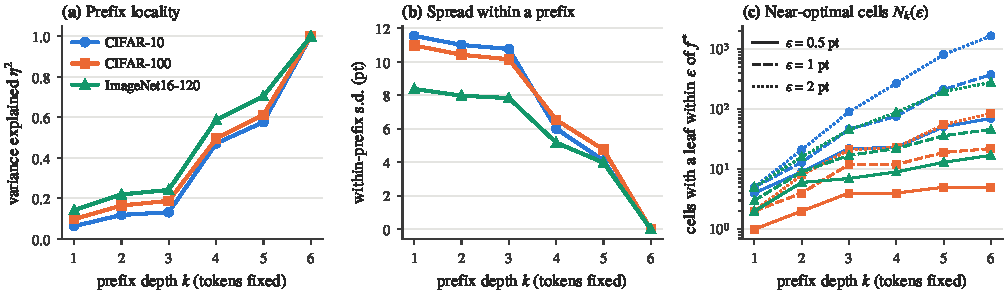
\includegraphics[width=\textwidth]{figs/figS3_landscape.pdf}
\caption{Landscape of NAS-Bench-201 seen through the trie. (a) Variance of validation accuracy explained by the first $k$ tokens. (b) Mean standard deviation of the architectures that share a prefix of length $k$. (c) Number of prefixes that still contain an architecture within $\varepsilon$ of the optimum (log scale). The first three tokens carry little information; locality appears from depth four.}
\label{f:landscape}
\end{figure}

\textit{Regret.} Figure~\ref{f:regret} shows the simple regret of every method against real evaluations at the largest budget, and Table~\ref{t:regretfit} the fitted power law $r_t\approx a\,t^{-b}$. Uniform sampling without replacement has $b$ = 0.29--0.46, and random, MCTS-style, ENAS-style, ZiCo-style search and LLM-NAS stay below 0.7. \rmg{} decays with $b$ = 1.74, 1.71 and 1.29 and reaches a final regret of 0.04, 0.08 and 0.15\,pt after 88--102 real evaluations; only local search decays clearly faster on CIFAR-10 and CIFAR-100 ($b$ = 2.68 and 3.24), where it reaches the optimum. The A7 trie arm reproduces \rmg{} exactly. The flat bandit with set deduplication has a similar exponent on CIFAR-10 (1.78) and a smaller one on CIFAR-100 and ImageNet16-120 (1.08, 0.90), although its final accuracy does not differ (section~\ref{s:abl}); the flat bandit without deduplication is slower still (1.12, 0.66, 0.74). The exponents are descriptive summaries over 25--200 evaluations, not asymptotic rates.

\begin{figure}[tbp]
\centering
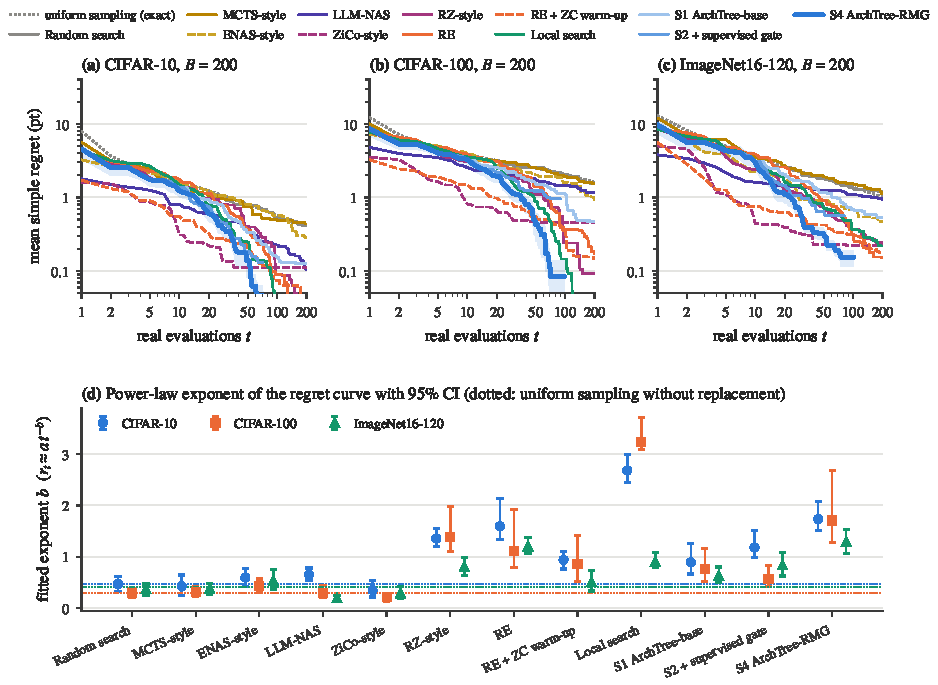
\includegraphics[width=\textwidth]{figs/figS2_regret.pdf}
\caption{Gap between the optimum of the space and the best validation accuracy found so far (simple regret), NAS-Bench-201, 200 proposals. (a)--(c) Mean of 12 seeds against real evaluations (log--log; band: $\pm$1 standard error for \rmg). Gated methods stop earlier because they spend fewer real evaluations. (d) Fitted exponent $b$ with 95\% bootstrap interval per method and dataset; dotted lines mark uniform sampling without replacement.}
\label{f:regret}
\end{figure}

\begin{table}[tbp]
\caption{Power-law fit of the regret curve at a budget of 200 proposals: real evaluations $T$ (maximum over seeds), exponent $b$ with 95\% bootstrap interval, and simple regret $r_T$ (pt) at $T$.}\label{t:regretfit}
\centering\scriptsize
\setlength{\tabcolsep}{3.5pt}
\begin{tabular}{@{}lrcrrcrrcr@{}}
\toprule
\multirow{2}{*}{Method} & \multicolumn{3}{c}{CIFAR-10} & \multicolumn{3}{c}{CIFAR-100} & \multicolumn{3}{c}{ImageNet16-120}\\
\cmidrule(lr){2-4}\cmidrule(lr){5-7}\cmidrule(lr){8-10}
 & $T$ & $b$ [95\% CI] & $r_T$ & $T$ & $b$ [95\% CI] & $r_T$ & $T$ & $b$ [95\% CI] & $r_T$\\
\midrule
Uniform sampling (exact) & 200 & 0.46 & 0.42 & 200 & 0.29 & 1.60 & 200 & 0.41 & 1.02\\
Random search & 200 & 0.47 [0.31, 0.61] & 0.41 & 200 & 0.30 [0.21, 0.39] & 1.55 & 200 & 0.37 [0.24, 0.46] & 1.22\\
MCTS-style & 200 & 0.42 [0.24, 0.64] & 0.44 & 200 & 0.31 [0.22, 0.42] & 1.55 & 200 & 0.37 [0.27, 0.48] & 1.13\\
ENAS-style & 200 & 0.59 [0.42, 0.77] & 0.28 & 200 & 0.43 [0.31, 0.56] & 0.95 & 200 & 0.53 [0.36, 0.74] & 0.48\\
LLM-NAS & 200 & 0.65 [0.54, 0.78] & 0.11 & 200 & 0.28 [0.20, 0.44] & 1.15 & 200 & 0.19 [0.14, 0.24] & 0.95\\
ZiCo-style & 200 & 0.34 [0.21, 0.53] & 0.11 & 200 & 0.21 [0.12, 0.29] & 0.46 & 200 & 0.28 [0.18, 0.41] & 0.22\\
RZ-style ZC walk & 200 & 1.35 [1.21, 1.56] & 0.04 & 200 & 1.38 [1.11, 1.98] & 0.09 & 200 & 0.79 [0.62, 0.99] & 0.25\\
RE & 200 & 1.59 [1.33, 2.14] & 0.02 & 200 & 1.11 [0.78, 1.93] & 0.17 & 200 & 1.20 [1.06, 1.38] & 0.15\\
RE + ZC warm-up & 200 & 0.94 [0.76, 1.11] & 0.03 & 200 & 0.86 [0.52, 1.42] & 0.15 & 200 & 0.50 [0.33, 0.72] & 0.18\\
Local search & 200 & 2.68 [2.45, 3.00] & 0.00 & 200 & 3.24 [3.09, 3.73] & 0.00 & 200 & 0.89 [0.78, 1.08] & 0.22\\
S1 ArchTree-base & 200 & 0.89 [0.66, 1.26] & 0.13 & 200 & 0.75 [0.51, 1.16] & 0.47 & 200 & 0.62 [0.50, 0.80] & 0.53\\
S2 (S1 + supervised gate) & 71 & 1.18 [0.98, 1.52] & 0.13 & 89 & 0.57 [0.42, 0.83] & 0.96 & 81 & 0.84 [0.62, 1.07] & 0.56\\
S4 ArchTree-RMG & 88 & 1.74 [1.51, 2.08] & 0.04 & 98 & 1.71 [1.28, 2.69] & 0.08 & 102 & 1.29 [1.07, 1.52] & 0.15\\
Flat UCB, no dedup (A7) & 142 & 1.12 [0.71, 1.76] & 0.11 & 148 & 0.66 [0.37, 1.31] & 0.66 & 144 & 0.74 [0.43, 1.17] & 0.55\\
Flat UCB + set dedup (A7) & 95 & 1.78 [1.47, 2.17] & 0.02 & 98 & 1.08 [0.96, 1.25] & 0.22 & 97 & 0.90 [0.72, 1.09] & 0.38\\
Trie (A7 arm) & 88 & 1.74 [1.51, 2.18] & 0.04 & 98 & 1.71 [1.27, 3.67] & 0.08 & 102 & 1.29 [1.03, 1.58] & 0.15\\
\bottomrule
\end{tabular}

\end{table}

%% =====================================================================
\section{Proxies, training cost and the gate-cost criterion}\label{s:proxy}

Table~\ref{t:calib} gives the rank correlation of each proxy with validation accuracy on the 1,500 calibration architectures. On NAS-Bench-201 the label-free ensemble $P$ is within 0.04 of the supervised ensemble in Kendall $\tau$ (0.63--0.68 against 0.63--0.72), and NASWOT is the best single proxy. On NAS-Bench-101 all proxies are weaker (best single $\tau$ = 0.39).

\begin{table}[tbp]
\caption{Rank correlation of each zero-cost proxy with validation accuracy (Kendall $\tau$, Spearman $\rho$; 1,500 architectures, calibration seed 0). $C$ is a cost proxy and enters only the cost-penalised gates.}\label{t:calib}
\centering\footnotesize
\begin{tabular}{@{}lrrrrrrrr@{}}
\toprule
\multirow{2}{*}{Proxy} & \multicolumn{2}{c}{NB201 C10} & \multicolumn{2}{c}{NB201 C100} & \multicolumn{2}{c}{NB201 IN16} & \multicolumn{2}{c}{NB101 C10}\\
\cmidrule(lr){2-3}\cmidrule(lr){4-5}\cmidrule(lr){6-7}\cmidrule(lr){8-9}
 & $\tau$ & $\rho$ & $\tau$ & $\rho$ & $\tau$ & $\rho$ & $\tau$ & $\rho$\\
\midrule
$E$ (SVD entropy) & 0.55 & 0.73 & 0.54 & 0.72 & 0.49 & 0.66 & 0.39 & 0.55\\
$S$ (SynFlow) & 0.55 & 0.75 & 0.59 & 0.78 & 0.56 & 0.74 & 0.26 & 0.38\\
$T$ (NASWOT) & 0.59 & 0.79 & 0.64 & 0.83 & 0.59 & 0.78 & 0.27 & 0.39\\
$C$ (FLOPs/params cost) & $-$0.50 & $-$0.69 & $-$0.53 & $-$0.72 & $-$0.48 & $-$0.66 & $-$0.37 & $-$0.54\\
supervised ensemble & 0.67 & 0.85 & 0.72 & 0.89 & 0.63 & 0.81 & 0.50 & 0.69\\
label-free ensemble $P$ & 0.64 & 0.83 & 0.68 & 0.86 & 0.63 & 0.81 & -- & --\\
\bottomrule
\end{tabular}

\end{table}

Table~\ref{t:costcorr} extends Figure~6(b) to every score and space. Two observations matter for the gate. First, in the cell spaces the label-free score, SynFlow and NASWOT are also cost proxies: the label-free score correlates with training time with $\rho$ = 0.78 (NB201) and 0.63 (NB101), so the admitted 35\% train 1.22 and 1.35 times longer than an average architecture. Measured against an oracle that admits the truly best 35\%, this over-payment is small on NAS-Bench-201 (3.4--5.1\%) but reaches 18.0\% on NAS-Bench-101. Second, in the width space of NATS-Bench SSS the correlation with cost is weak ($\rho$ = 0.20--0.21) and the admitted set is cheaper than the oracle set ($-$1.7 to $-$6.4\%). The parameter count, often used as a free gate, is tied to cost as strongly as or more strongly than any accuracy proxy ($\rho$ = 0.68--0.87).

\begin{table}[tbp]
\caption{Correlation of every gate score with training time $\tau$ (Spearman $\rho$) and with validation accuracy $A$ (Kendall $\tau_K$) over the space (NB201: all 15,625 architectures; NB101 and NATS-SSS: 2,000 random architectures), mean training time of the top 35\% relative to the space average, excess of that cost over the oracle top 35\%, and mean validation accuracy of the admitted architectures.}\label{t:costcorr}
\centering\footnotesize
\begin{tabular}{@{}llrrrrr@{}}
\toprule
Space & Score & $\rho$(score, $\tau$) & $\tau_K$(score, $A$) & cost ratio of top 35\% & excess vs oracle (\%) & mean $A$ of top 35\%\\
\midrule
NB201 C10 & $E$ & 0.44 & 0.55 & 1.13 & $-$3.1 & 88.54\\
 & $S$ & 0.75 & 0.55 & 1.21 & 4.0 & 88.70\\
 & $T$ & 0.82 & 0.59 & 1.23 & 6.3 & 88.83\\
 & $C$ & $-$0.88 & $-$0.49 & 0.76 & $-$34.8 & 77.99\\
 & $P$ (label-free) & 0.78 & 0.64 & 1.22 & 5.1 & 88.90\\
 & \#params & 0.83 & 0.53 & 1.21 & 4.6 & 87.80\\
 & val. acc. (oracle) & 0.59 & 1.00 & 1.16 & 0.0 & 89.39\\
\midrule
NB201 C100 & $E$ & 0.44 & 0.54 & 1.13 & $-$4.7 & 67.15\\
 & $S$ & 0.75 & 0.58 & 1.21 & 2.3 & 67.67\\
 & $T$ & 0.82 & 0.63 & 1.23 & 4.6 & 67.92\\
 & $C$ & $-$0.88 & $-$0.51 & 0.76 & $-$35.9 & 54.40\\
 & $P$ (label-free) & 0.78 & 0.67 & 1.22 & 3.4 & 68.00\\
 & \#params & 0.83 & 0.55 & 1.21 & 2.9 & 66.62\\
 & val. acc. (oracle) & 0.65 & 1.00 & 1.18 & 0.0 & 68.67\\
\midrule
NB201 IN16 & $E$ & 0.44 & 0.49 & 1.13 & $-$3.3 & 39.04\\
 & $S$ & 0.75 & 0.56 & 1.21 & 3.8 & 39.79\\
 & $T$ & 0.82 & 0.59 & 1.23 & 6.1 & 40.15\\
 & $C$ & $-$0.88 & $-$0.47 & 0.76 & $-$34.9 & 27.76\\
 & $P$ (label-free) & 0.78 & 0.64 & 1.22 & 4.9 & 40.18\\
 & \#params & 0.83 & 0.51 & 1.21 & 4.4 & 38.69\\
 & val. acc. (oracle) & 0.60 & 1.00 & 1.16 & 0.0 & 41.56\\
\midrule
NB101 C10 & $E$ & 0.10 & 0.38 & 1.05 & $-$8.2 & 91.70\\
 & $S$ & 0.63 & 0.23 & 1.36 & 18.5 & 91.34\\
 & $T$ & 0.82 & 0.23 & 1.48 & 29.0 & 90.86\\
 & $C$ & $-$0.42 & $-$0.38 & 0.80 & $-$29.8 & 88.05\\
 & $P$ (label-free) & 0.63 & 0.33 & 1.35 & 18.0 & 91.46\\
 & \#params & 0.87 & 0.29 & 1.48 & 29.2 & 91.23\\
 & val. acc. (oracle) & 0.33 & 1.00 & 1.14 & 0.0 & 92.88\\
\midrule
NATS-SSS C10 & $E$ & 0.13 & 0.34 & 1.03 & $-$7.5 & 88.62\\
 & $S$ & 0.27 & 0.63 & 1.05 & $-$5.2 & 89.00\\
 & $T$ & 0.11 & 0.35 & 1.02 & $-$8.0 & 88.58\\
 & $C$ & $-$0.25 & $-$0.57 & 0.95 & $-$14.6 & 86.92\\
 & $P$ (label-free) & 0.20 & 0.53 & 1.04 & $-$6.4 & 88.89\\
 & \#params & 0.74 & 0.69 & 1.15 & 3.0 & 89.04\\
 & val. acc. (oracle) & 0.59 & 1.00 & 1.11 & 0.0 & 89.17\\
\midrule
NATS-SSS C100 & $E$ & 0.13 & 0.56 & 1.03 & $-$3.7 & 66.32\\
 & $S$ & 0.27 & 0.79 & 1.06 & $-$1.1 & 67.20\\
 & $T$ & 0.11 & 0.24 & 1.02 & $-$4.3 & 64.49\\
 & $C$ & $-$0.25 & $-$0.65 & 0.95 & $-$11.4 & 58.17\\
 & $P$ (label-free) & 0.20 & 0.63 & 1.04 & $-$2.4 & 66.80\\
 & \#params & 0.74 & 0.54 & 1.15 & 7.9 & 66.28\\
 & val. acc. (oracle) & 0.29 & 1.00 & 1.07 & 0.0 & 67.41\\
\midrule
NATS-SSS IN16 & $E$ & 0.14 & 0.49 & 1.01 & $-$2.2 & 40.32\\
 & $S$ & 0.27 & 0.74 & 1.02 & $-$1.3 & 41.46\\
 & $T$ & 0.14 & 0.29 & 1.01 & $-$2.2 & 39.26\\
 & $C$ & $-$0.27 & $-$0.58 & 0.98 & $-$5.0 & 33.61\\
 & $P$ (label-free) & 0.21 & 0.62 & 1.02 & $-$1.7 & 41.09\\
 & \#params & 0.68 & 0.65 & 1.05 & 1.3 & 41.14\\
 & val. acc. (oracle) & 0.46 & 1.00 & 1.03 & 0.0 & 41.80\\
\bottomrule
\end{tabular}

\end{table}

\textit{Gate-cost criterion.} Table~\ref{t:gatecost} gives all six normal-score correlations behind Eq.~7 together with the predicted and measured effect of a cost penalty $\lambda=1$, and Figure~\ref{f:gatecost} compares prediction and measurement for each of the 75 measured cells. The criterion is negative in all seven spaces and the measured effect is negative in all seven; across cells the predicted and measured changes are rank-correlated ($\rho$ = 0.81 over both $\lambda$ values, 0.71 for $\lambda=1$ alone) and agree in sign in 53 of 75 cells, including all 39 cells with $\lambda=1$; all 22 disagreements are $\lambda=0.25$ cells in which the predicted change lies within $\pm$0.02\,pt although the measured loss reaches up to 0.99\,pt. The Gaussian-copula model underestimates the size of the loss by a factor of about 4 to 10, because the gate acts on the upper tail of the score distribution, where the dependence between proxy and accuracy is stronger than a single correlation describes. The criterion should therefore be read as a test of direction, not as a forecast of magnitude.

\begin{table}[tbp]
\caption{Gate-cost model per space: normal-score correlations between gate score $P$, accuracy $A$, predicted cost $D=\log(1+\#\text{params})$ and recorded training time $C$; criterion slope $r_{PA}r_{PD}-r_{DA}$ at $\lambda=0$; predicted and measured change (pt) of test accuracy at equal GPU-hours for $\lambda=1$ (mean over $k$ and proposers).}\label{t:gatecost}
\centering\footnotesize
\begin{tabular}{@{}lrrrrrrrrr@{}}
\toprule
Space & $r_{PA}$ & $r_{PD}$ & $r_{DA}$ & $r_{PC}$ & $r_{AC}$ & $r_{DC}$ & slope & pred. $\Delta$ & meas. $\Delta$\\
\midrule
NB201 C10 & 0.83 & 0.79 & 0.69 & 0.77 & 0.59 & 0.85 & $-$0.037 & $-$0.07 & $-$0.48\\
NB201 C100 & 0.86 & 0.79 & 0.72 & 0.77 & 0.65 & 0.85 & $-$0.043 & $-$0.22 & $-$1.02\\
NB201 IN16 & 0.82 & 0.79 & 0.66 & 0.77 & 0.61 & 0.85 & $-$0.019 & $-$0.15 & $-$1.14\\
NB101 C10 & 0.47 & 0.82 & 0.44 & 0.65 & 0.35 & 0.89 & $-$0.049 & $-$0.03 & $-$0.30\\
NATS-SSS C10 & 0.74 & 0.67 & 0.89 & 0.23 & 0.62 & 0.76 & $-$0.390 & $-$0.13 & $-$0.47\\
NATS-SSS C100 & 0.84 & 0.67 & 0.75 & 0.23 & 0.33 & 0.77 & $-$0.185 & $-$0.11 & $-$0.95\\
NATS-SSS IN16 & 0.83 & 0.67 & 0.85 & 0.21 & 0.46 & 0.66 & $-$0.293 & $-$0.50 & $-$1.92\\
\bottomrule
\end{tabular}

\end{table}

\begin{figure}[tbp]
\centering
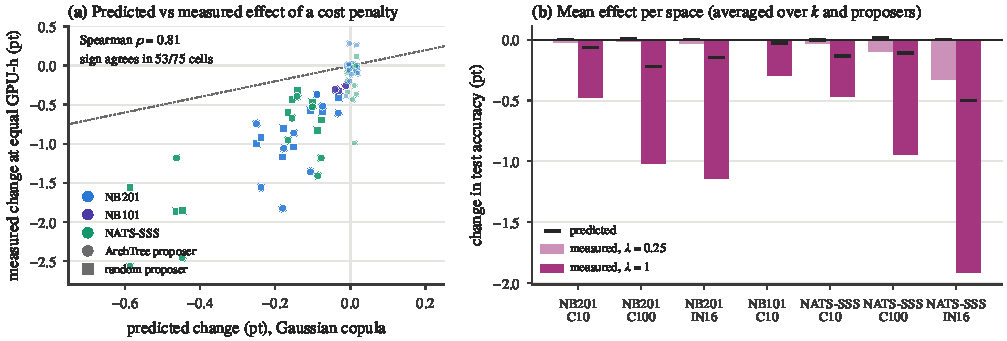
\includegraphics[width=\textwidth]{figs/figS9_gatecost_validation.pdf}
\caption{Validation of the gate-cost criterion. (a) Predicted against measured change in test accuracy when a cost penalty is added to the gate, for every benchmark, dataset, budget $k$, proposer and $\lambda$ (large markers: $\lambda=1$; small: $\lambda=0.25$); the dotted line is $y=x$. (b) Mean measured change per space (bars) and the corresponding prediction (black ticks). Every space predicts and shows a loss.}
\label{f:gatecost}
\end{figure}

%% =====================================================================
\section{Fixed proposal budget: all cells}\label{s:fixed}

Table~\ref{t:mainfull} gives every method on every dataset and budget; Table~4 of the main paper is its last column. Table~\ref{t:fixedtests} and Figure~\ref{f:fixedtests} summarise the 132 paired comparisons of \rmg{} with each baseline. Two definitions of equal effort are used: the same number of proposals, which favours ungated methods since they evaluate every proposal, and a budget at which the baseline receives at least as many real evaluations as \rmg{} used. The second definition changes the counts only slightly (21 wins and no loss against the external baselines). Against the nine external baselines \rmg{} has 20 wins and no loss in 108 comparisons: 7 against random search, 6 against MCTS-style search, 3 each against ENAS-style search and LLM-NAS, and 1 against ZiCo-style search. Against RE with a ZC warm-up and local search the mean difference is slightly negative ($-$0.22 and $-$0.08\,pt) but never significant.

\begin{table}[tbp]
\caption{NAS-Bench-201: test accuracy (mean $\pm$ standard deviation over 12 seeds) of the best-validation architecture at each proposal budget $B$. Best value per column in bold.}\label{t:mainfull}
\centering\footnotesize
\setlength{\tabcolsep}{5pt}
\begin{tabular}{@{}lcccc@{}}
\toprule
Method & $B$ = 25 & $B$ = 50 & $B$ = 100 & $B$ = 200\\
\midrule
\multicolumn{5}{@{}l}{\textit{CIFAR-10}}\\
\quad Random search & 93.45 $\pm$ 0.45 & 93.62 $\pm$ 0.21 & 93.82 $\pm$ 0.30 & 93.92 $\pm$ 0.21\\
\quad MCTS-style & 93.55 $\pm$ 0.36 & 93.68 $\pm$ 0.27 & 93.89 $\pm$ 0.15 & 93.89 $\pm$ 0.20\\
\quad ENAS-style & 93.43 $\pm$ 0.71 & 93.68 $\pm$ 0.48 & 93.74 $\pm$ 0.41 & 94.09 $\pm$ 0.26\\
\quad LLM-NAS & 93.93 $\pm$ 0.21 & 93.99 $\pm$ 0.25 & 94.04 $\pm$ 0.19 & 94.28 $\pm$ 0.08\\
\quad ZiCo-style & \textbf{93.93 $\pm$ 0.22} & 94.08 $\pm$ 0.20 & 94.17 $\pm$ 0.18 & 94.29 $\pm$ 0.12\\
\quad RZ-style ZC walk & 93.72 $\pm$ 0.27 & 94.06 $\pm$ 0.21 & \textbf{94.28 $\pm$ 0.11} & 94.33 $\pm$ 0.07\\
\quad RE & 93.42 $\pm$ 0.41 & 93.94 $\pm$ 0.36 & 94.17 $\pm$ 0.24 & 94.31 $\pm$ 0.13\\
\quad RE + ZC warm-up & 93.91 $\pm$ 0.33 & \textbf{94.26 $\pm$ 0.15} & 94.22 $\pm$ 0.19 & 94.28 $\pm$ 0.19\\
\quad Local search & 93.75 $\pm$ 0.43 & 93.97 $\pm$ 0.38 & 94.27 $\pm$ 0.22 & \textbf{94.37 $\pm$ 0.00}\\
\quad S1 ArchTree-base & 93.64 $\pm$ 0.43 & 93.99 $\pm$ 0.19 & 94.09 $\pm$ 0.24 & 94.11 $\pm$ 0.26\\
\quad S2 (S1 + supervised gate) & 93.60 $\pm$ 0.44 & 93.98 $\pm$ 0.34 & 94.15 $\pm$ 0.25 & 94.17 $\pm$ 0.22\\
\quad S4 ArchTree-RMG & 93.60 $\pm$ 0.31 & 94.04 $\pm$ 0.27 & 94.19 $\pm$ 0.26 & 94.28 $\pm$ 0.13\\
\midrule
\multicolumn{5}{@{}l}{\textit{CIFAR-100}}\\
\quad Random search & 70.84 $\pm$ 0.64 & 71.06 $\pm$ 0.78 & 71.54 $\pm$ 0.83 & 71.92 $\pm$ 0.81\\
\quad MCTS-style & 70.59 $\pm$ 0.98 & 70.97 $\pm$ 0.91 & 71.62 $\pm$ 0.69 & 71.94 $\pm$ 0.87\\
\quad ENAS-style & 71.02 $\pm$ 1.25 & 71.58 $\pm$ 1.14 & 71.79 $\pm$ 1.15 & 72.59 $\pm$ 0.81\\
\quad LLM-NAS & 71.36 $\pm$ 0.51 & 71.39 $\pm$ 0.42 & 71.96 $\pm$ 0.28 & 72.14 $\pm$ 0.43\\
\quad ZiCo-style & 71.93 $\pm$ 0.80 & 72.33 $\pm$ 0.66 & 72.68 $\pm$ 0.58 & 72.97 $\pm$ 0.43\\
\quad RZ-style ZC walk & 71.39 $\pm$ 0.77 & 72.17 $\pm$ 0.99 & 73.20 $\pm$ 0.35 & 73.39 $\pm$ 0.19\\
\quad RE & 70.43 $\pm$ 1.22 & 71.61 $\pm$ 1.21 & 72.96 $\pm$ 0.78 & 73.37 $\pm$ 0.21\\
\quad RE + ZC warm-up & \textbf{72.00 $\pm$ 1.03} & \textbf{72.92 $\pm$ 0.56} & 73.13 $\pm$ 0.50 & 73.36 $\pm$ 0.23\\
\quad Local search & 71.44 $\pm$ 1.48 & 72.63 $\pm$ 1.09 & \textbf{73.36 $\pm$ 0.42} & \textbf{73.51 $\pm$ 0.00}\\
\quad S1 ArchTree-base & 71.12 $\pm$ 1.35 & 72.06 $\pm$ 0.93 & 72.50 $\pm$ 0.85 & 73.12 $\pm$ 0.45\\
\quad S2 (S1 + supervised gate) & 70.98 $\pm$ 1.40 & 71.46 $\pm$ 1.37 & 72.26 $\pm$ 1.06 & 72.45 $\pm$ 0.89\\
\quad S4 ArchTree-RMG & 71.51 $\pm$ 1.26 & 72.19 $\pm$ 0.91 & 73.02 $\pm$ 0.75 & 73.40 $\pm$ 0.20\\
\midrule
\multicolumn{5}{@{}l}{\textit{ImageNet16-120}}\\
\quad Random search & 44.74 $\pm$ 1.25 & 45.15 $\pm$ 0.73 & 45.49 $\pm$ 0.85 & 45.47 $\pm$ 0.80\\
\quad MCTS-style & 44.24 $\pm$ 1.03 & 44.66 $\pm$ 0.99 & 45.14 $\pm$ 0.86 & 45.44 $\pm$ 0.65\\
\quad ENAS-style & 45.26 $\pm$ 1.12 & 45.84 $\pm$ 0.78 & 46.04 $\pm$ 0.44 & 46.16 $\pm$ 0.36\\
\quad LLM-NAS & 44.77 $\pm$ 0.34 & 45.35 $\pm$ 0.54 & 45.29 $\pm$ 0.30 & 45.37 $\pm$ 0.36\\
\quad ZiCo-style & 45.37 $\pm$ 1.04 & 46.11 $\pm$ 0.48 & 46.22 $\pm$ 0.42 & 46.28 $\pm$ 0.57\\
\quad RZ-style ZC walk & 45.53 $\pm$ 0.89 & 46.06 $\pm$ 0.46 & 46.22 $\pm$ 0.45 & 46.32 $\pm$ 0.18\\
\quad RE & 44.53 $\pm$ 1.35 & 45.67 $\pm$ 1.10 & \textbf{46.51 $\pm$ 0.29} & 46.48 $\pm$ 0.17\\
\quad RE + ZC warm-up & \textbf{46.11 $\pm$ 0.57} & \textbf{46.31 $\pm$ 0.53} & 46.14 $\pm$ 0.57 & 46.34 $\pm$ 0.36\\
\quad Local search & 45.23 $\pm$ 0.96 & 46.05 $\pm$ 0.79 & 46.11 $\pm$ 0.65 & \textbf{46.52 $\pm$ 0.29}\\
\quad S1 ArchTree-base & 44.93 $\pm$ 1.08 & 45.70 $\pm$ 0.58 & 46.11 $\pm$ 0.46 & 46.25 $\pm$ 0.40\\
\quad S2 (S1 + supervised gate) & 44.90 $\pm$ 1.23 & 45.72 $\pm$ 1.08 & 45.81 $\pm$ 0.93 & 46.39 $\pm$ 0.51\\
\quad S4 ArchTree-RMG & 45.28 $\pm$ 1.07 & 45.91 $\pm$ 0.51 & 46.45 $\pm$ 0.39 & 46.41 $\pm$ 0.18\\
\bottomrule
\end{tabular}

\end{table}

\begin{table}[tbp]
\caption{Paired comparison of \rmg{} with each baseline over the 12 dataset--budget cells: Holm-corrected W/T/L (Holm within baseline), range and mean of the paired difference $\Delta$ (pt, \rmg{} minus baseline) and median Cohen's $d$; on the right, the same comparison when each baseline is given at least as many real evaluations as \rmg{} used.}\label{t:fixedtests}
\centering\footnotesize
\begin{tabular}{@{}lcccccc@{}}
\toprule
\multirow{2}{*}{Baseline} & \multicolumn{4}{c}{Same proposal budget (12 cells)} & \multicolumn{2}{c}{Matched real evaluations (12 cells)}\\
\cmidrule(lr){2-5}\cmidrule(lr){6-7}
 & W/T/L & range of $\Delta$ & mean $\Delta$ & median $d$ & W/T/L & mean $\Delta$\\
\midrule
Random search & 7/5/0 & 0.14 to 1.48 & 0.77 & 1.01 & 7/5/0 & 0.81\\
MCTS-style & 6/6/0 & 0.05 to 1.47 & 0.89 & 1.05 & 6/6/0 & 0.92\\
ENAS-style & 3/9/0 & 0.01 to 1.23 & 0.42 & 0.60 & 4/8/0 & 0.52\\
LLM-NAS & 3/9/0 & $-$0.33 to 1.27 & 0.53 & 0.57 & 3/9/0 & 0.57\\
ZiCo-style & 1/11/0 & $-$0.42 to 0.43 & $-$0.01 & $-$0.04 & 1/11/0 & 0.03\\
RZ-style ZC walk & 0/12/0 & $-$0.25 to 0.23 & $-$0.03 & $-$0.11 & 0/12/0 & $-$0.01\\
RE & 0/12/0 & $-$0.07 to 1.08 & 0.24 & 0.15 & 0/12/0 & 0.29\\
RE + ZC warm-up & 0/12/0 & $-$0.83 to 0.31 & $-$0.22 & $-$0.22 & 0/12/0 & $-$0.20\\
Local search & 0/12/0 & $-$0.44 to 0.35 & $-$0.08 & $-$0.24 & 0/12/0 & $-$0.06\\
S1 ArchTree-base & 0/12/0 & $-$0.04 to 0.52 & 0.22 & 0.37 & 1/11/0 & 0.27\\
S2 (S1 + supervised gate) & 1/11/0 & 0.00 to 0.96 & 0.37 & 0.39 & 1/11/0 & 0.38\\
\bottomrule
\end{tabular}

\end{table}

\begin{figure}[tbp]
\centering
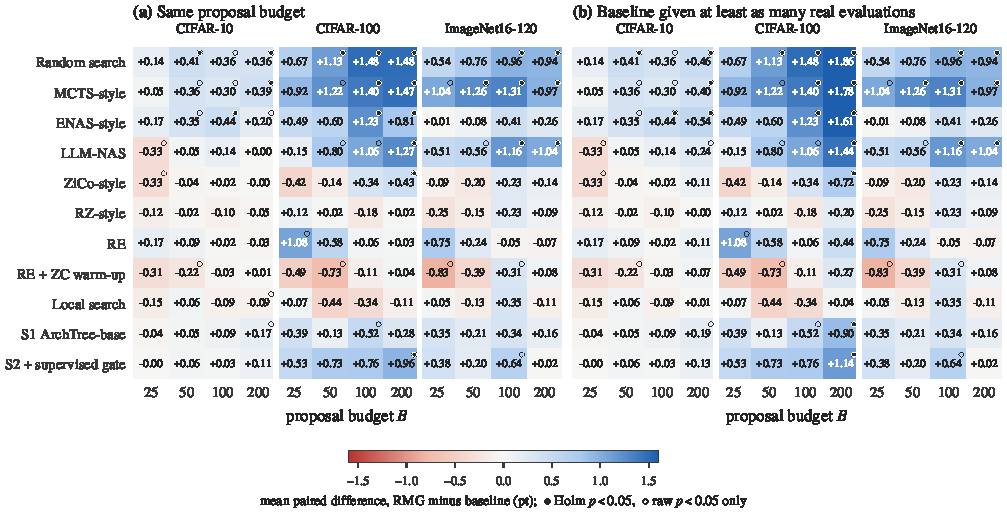
\includegraphics[width=\textwidth]{figs/figS4_fixed_tests.pdf}
\caption{Mean paired difference in test accuracy between \rmg{} and each baseline on NAS-Bench-201 (blue: \rmg{} better). Filled dots: significant after Holm correction within the baseline; open dots: $p<0.05$ before correction only. (a) Same number of proposals. (b) Baseline budget raised until it receives at least as many real evaluations as \rmg.}
\label{f:fixedtests}
\end{figure}

\textit{Repeated evaluations.} Table~\ref{t:dups} and Figure~\ref{f:dups} count real evaluations of architectures that the same run had already trained. All \algname{} variants have none (statement T2), as do the population and sampling baselines that keep a history. The LLM generator repeats itself increasingly as the budget grows (6.4\% at 25 proposals, 55.4\% at 200, up to 133 repeats in one run), and a flat bandit that keeps no memory wastes 60--75\% of its evaluations on architectures it has already trained, which is the waste that deduplication removes.

\begin{table}[tbp]
\caption{Repeated real evaluations: mean share over runs (\%) and maximum number in a single run, per proposal budget $B$ (NAS-Bench-201, mean over the three datasets).}\label{t:dups}
\centering\footnotesize
\begin{tabular}{@{}lrrrrrrrr@{}}
\toprule
\multirow{2}{*}{Method} & \multicolumn{2}{c}{$B$ = 25} & \multicolumn{2}{c}{$B$ = 50} & \multicolumn{2}{c}{$B$ = 100} & \multicolumn{2}{c}{$B$ = 200}\\
\cmidrule(lr){2-3}\cmidrule(lr){4-5}\cmidrule(lr){6-7}\cmidrule(lr){8-9}
 & \% & max & \% & max & \% & max & \% & max\\
\midrule
Random search & 0.0 & 0 & 0.0 & 0 & 0.0 & 0 & 0.0 & 0\\
MCTS-style & 0.2 & 1 & 0.2 & 1 & 0.2 & 1 & 0.3 & 3\\
ENAS-style & 0.0 & 0 & 0.0 & 0 & 0.0 & 0 & 0.0 & 0\\
LLM-NAS & 6.4 & 5 & 20.3 & 18 & 36.9 & 49 & 55.4 & 133\\
ZiCo-style & 0.0 & 0 & 0.0 & 0 & 0.0 & 0 & 0.0 & 0\\
RZ-style ZC walk & 0.0 & 0 & 0.0 & 0 & 0.0 & 0 & 0.0 & 0\\
RE & 0.0 & 0 & 0.0 & 0 & 0.0 & 0 & 0.0 & 0\\
RE + ZC warm-up & 0.0 & 0 & 0.0 & 0 & 0.0 & 0 & 0.0 & 0\\
Local search & 0.0 & 0 & 0.0 & 0 & 0.0 & 0 & 0.0 & 0\\
S1 ArchTree-base & 0.0 & 0 & 0.0 & 0 & 0.0 & 0 & 0.0 & 0\\
S2 (S1 + supervised gate) & 0.0 & 0 & 0.0 & 0 & 0.0 & 0 & 0.0 & 0\\
S4 ArchTree-RMG & 0.0 & 0 & 0.0 & 0 & 0.0 & 0 & 0.0 & 0\\
Flat UCB, no dedup (A7) & 60.4 & 14 & 64.4 & 28 & 68.9 & 56 & 74.5 & 109\\
Flat UCB + set dedup (A7) & 0.0 & 0 & 0.0 & 0 & 0.0 & 0 & 0.0 & 0\\
Trie (A7 arm) & 0.0 & 0 & 0.0 & 0 & 0.0 & 0 & 0.0 & 0\\
\bottomrule
\end{tabular}

\end{table}

\begin{figure}[tbp]
\centering
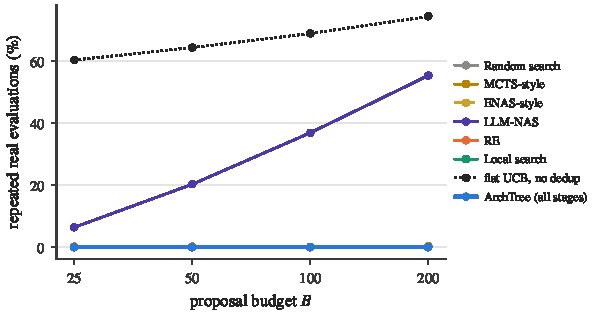
\includegraphics[width=0.6\textwidth]{figs/figS16_duplicates.pdf}
\caption{Share of real evaluations spent on architectures already evaluated in the same run (NAS-Bench-201, mean over datasets and seeds). Methods not shown, and all \algname{} stages, stay at or below 0.3\%.}
\label{f:dups}
\end{figure}

%% =====================================================================
\section{Equal GPU-hours: all cells}\label{s:egh}

Tables~\ref{t:egh201}, \ref{t:eghnats} and \ref{t:egh101} list the mean test accuracy of every arm in every cell of the equal-GPU-hour protocol (Eq.~8), with a marker where \rmg{} is significantly better. Table~\ref{t:eghwtl} counts the outcomes per comparator and benchmark, and Figure~\ref{f:egh} shows every paired difference. \rmg{} has 57 wins and no loss in 261 comparisons (38/79/0 on NAS-Bench-201, 4/23/0 on NAS-Bench-101 and 15/102/0 on NATS-Bench SSS). Most wins are against ungated random search (10) and the two $\lambda=1$ cost penalties (31); on NAS-Bench-201 they also include random search with the label-free gate or with $\lambda=0.25$ (6 each), the ungated \algname-RM (2), ungated RE (1) and the parameter-count gate (1). Against the other gated arms, RE with the ZC warm-up and local search, the mean differences lie between $-$0.24 and $+$0.41\,pt, with a single significant cell (the parameter-count gate on NAS-Bench-201). Five of the 1,128 runs ran out of proposals before their GPU-hour budget was spent (all \algname-RM with $\lambda=1$ on NAS-Bench-101 at $k=100$, seeds 111, 789, 999, 1001 and 2024); they are kept with the accuracy they reached.

\begin{table}[tbp]
\caption{NAS-Bench-201 at equal GPU-hours: mean test accuracy for budget $H_k=k\bar\tau$. Bold: best arm in the column; $^{\triangledown}$: \rmg{} significantly better ($p_{\mathrm{Holm}}<0.05$). No arm is significantly better than \rmg{} in any cell.}\label{t:egh201}
\centering\footnotesize
\begin{tabular}{@{}lrrrrrrrrr@{}}
\toprule
\multirow{2}{*}{Arm} & \multicolumn{3}{c}{CIFAR-10} & \multicolumn{3}{c}{CIFAR-100} & \multicolumn{3}{c}{ImageNet16-120}\\
\cmidrule(lr){2-4}\cmidrule(lr){5-7}\cmidrule(lr){8-10}
 & 25 & 50 & 100 & 25 & 50 & 100 & 25 & 50 & 100\\
\midrule
ArchTree-RMG & 93.83 & 94.11 & 94.28 & 72.09 & 72.60 & 73.40 & 45.45 & \textbf{46.49} & 46.41\\
ArchTree-RM (no gate) & 93.64 & 93.79$^{\triangledown}$ & 94.09 & 71.28 & 72.07 & 72.84 & 45.10 & 45.56$^{\triangledown}$ & 45.91\\
ArchTree-RM + \#params gate & 93.81 & 94.15 & 94.25 & 71.82 & 72.40 & 73.21 & 45.44 & 46.01$^{\triangledown}$ & 46.32\\
ArchTree-RM + cost pen. ($\lambda$=0.25) & 93.75 & 94.13 & 94.17 & 71.99 & 72.88 & 73.20 & 45.71 & 46.10 & 46.35\\
ArchTree-RM + cost pen. ($\lambda$=1) & 93.45$^{\triangledown}$ & 93.59$^{\triangledown}$ & 93.67$^{\triangledown}$ & 71.03 & 71.85 & 71.85$^{\triangledown}$ & 44.58 & 44.67$^{\triangledown}$ & 45.05$^{\triangledown}$\\
RE + gate & 93.67 & 94.16 & 94.35 & 71.43 & 72.71 & 73.28 & 44.97 & 45.79 & 46.39\\
RE + ZC warm-up & \textbf{94.10} & \textbf{94.20} & 94.24 & \textbf{72.56} & 72.88 & 73.05 & \textbf{45.88} & 45.95 & 46.16\\
RE & 93.55 & 93.90 & 94.08 & 70.77$^{\triangledown}$ & 71.48 & 72.76 & 45.06 & 46.04 & 46.24\\
LS + gate & 93.78 & 94.08 & \textbf{94.37} & 71.29 & \textbf{72.90} & \textbf{73.51} & 45.04 & 45.61 & \textbf{46.47}\\
LS & 93.68 & 93.94 & 94.19 & 70.77 & 72.09 & 73.14 & 45.17 & 45.75 & 46.25\\
Random + gate & 93.62 & 93.83 & 93.92$^{\triangledown}$ & 71.06$^{\triangledown}$ & 71.56$^{\triangledown}$ & 71.92$^{\triangledown}$ & 45.09 & 45.49$^{\triangledown}$ & 45.45$^{\triangledown}$\\
Random & 93.45 & 93.62$^{\triangledown}$ & 93.82$^{\triangledown}$ & 70.84$^{\triangledown}$ & 71.06$^{\triangledown}$ & 71.54$^{\triangledown}$ & 44.71 & 45.15$^{\triangledown}$ & 45.53$^{\triangledown}$\\
Random + cost pen. ($\lambda$=0.25) & 93.60 & 93.83 & 93.95$^{\triangledown}$ & 71.03$^{\triangledown}$ & 71.54$^{\triangledown}$ & 71.92$^{\triangledown}$ & 45.10 & 45.49$^{\triangledown}$ & 45.45$^{\triangledown}$\\
Random + cost pen. ($\lambda$=1) & 93.26$^{\triangledown}$ & 93.25$^{\triangledown}$ & 93.52$^{\triangledown}$ & 70.25$^{\triangledown}$ & 70.56$^{\triangledown}$ & 71.00$^{\triangledown}$ & 44.05$^{\triangledown}$ & 44.32$^{\triangledown}$ & 44.87$^{\triangledown}$\\
\bottomrule
\end{tabular}

\end{table}

\begin{table}[tbp]
\caption{NATS-Bench SSS at equal GPU-hours (same layout as Table~\ref{t:egh201}).}\label{t:eghnats}
\centering\footnotesize
\begin{tabular}{@{}lrrrrrrrrr@{}}
\toprule
\multirow{2}{*}{Arm} & \multicolumn{3}{c}{CIFAR-10} & \multicolumn{3}{c}{CIFAR-100} & \multicolumn{3}{c}{ImageNet16-120}\\
\cmidrule(lr){2-4}\cmidrule(lr){5-7}\cmidrule(lr){8-10}
 & 25 & 50 & 100 & 25 & 50 & 100 & 25 & 50 & 100\\
\midrule
ArchTree-RMG & 92.95 & 93.24 & 93.18 & 69.58 & 69.83 & 70.23 & 44.46 & 45.60 & 45.62\\
ArchTree-RM (no gate) & 92.65 & 92.88 & 93.05 & 69.10 & 69.46 & 69.82 & 44.04 & 44.99 & 45.36\\
ArchTree-RM + \#params gate & 93.00 & 93.07 & 93.25 & 69.64 & 69.69 & 70.19 & 44.78 & 45.23 & 45.46\\
ArchTree-RM + cost pen. ($\lambda$=0.25) & 92.85 & 93.17 & 93.15 & 69.33 & 69.83 & 69.86 & 44.26 & 44.61 & 45.18\\
ArchTree-RM + cost pen. ($\lambda$=1) & 92.55$^{\triangledown}$ & 92.56$^{\triangledown}$ & 92.65$^{\triangledown}$ & 68.63$^{\triangledown}$ & 68.65$^{\triangledown}$ & 68.82$^{\triangledown}$ & 43.28$^{\triangledown}$ & 43.03$^{\triangledown}$ & 43.16$^{\triangledown}$\\
RE + gate & 93.02 & 93.14 & \textbf{93.36} & 69.48 & 69.76 & \textbf{70.34} & 44.75 & 45.26 & 45.51\\
RE + ZC warm-up & 93.14 & 93.18 & 93.18 & 69.64 & 69.86 & 70.13 & 45.39 & \textbf{45.87} & 45.69\\
RE & 92.91 & 93.03 & 93.25 & 69.00 & 69.70 & 69.94 & 44.17 & 44.91 & 45.46\\
LS + gate & \textbf{93.17} & \textbf{93.29} & 93.32 & \textbf{69.76} & \textbf{70.13} & 70.16 & \textbf{45.41} & 45.84 & \textbf{45.75}\\
LS & 93.09 & 93.20 & 93.34 & 69.74 & 69.95 & 70.14 & 44.67 & 45.76 & 45.50\\
Random + gate & 92.97 & 93.10 & 93.10 & 69.26 & 69.40 & 69.69 & 44.90 & 44.81 & 45.26\\
Random & 92.99 & 92.97 & 93.08 & 69.17 & 69.43 & 69.33 & 44.40 & 44.74 & 44.71\\
Random + cost pen. ($\lambda$=0.25) & 92.97 & 93.07 & 93.12 & 69.26 & 69.31 & 69.81 & 44.56 & 44.81 & 45.26\\
Random + cost pen. ($\lambda$=1) & 92.65 & 92.66$^{\triangledown}$ & 92.63$^{\triangledown}$ & 68.66 & 68.71$^{\triangledown}$ & 68.86$^{\triangledown}$ & 43.03 & 43.24$^{\triangledown}$ & 43.41$^{\triangledown}$\\
\bottomrule
\end{tabular}

\end{table}

\begin{table}[tbp]
\caption{NAS-Bench-101 (CIFAR-10) at equal GPU-hours: mean $\pm$ standard deviation of test accuracy and mean number of real evaluations that fit into each budget. Markers as in Table~\ref{t:egh201}.}\label{t:egh101}
\centering\footnotesize
\begin{tabular}{@{}lcccc@{}}
\toprule
Arm & $k$ = 25 & $k$ = 50 & $k$ = 100 & real evals ($k$ = 25 / 50 / 100)\\
\midrule
ArchTree-RMG & \textbf{93.63 $\pm$ 0.20} & 93.71 $\pm$ 0.18 & 93.82 $\pm$ 0.18 & 27 / 48 / 88\\
ArchTree-RM (no gate) & 93.49 $\pm$ 0.26 & 93.56 $\pm$ 0.21 & 93.78 $\pm$ 0.24 & 32 / 60 / 116\\
ArchTree-RM + \#params gate & 93.47 $\pm$ 0.21 & 93.60 $\pm$ 0.14 & 93.93 $\pm$ 0.22 & 26 / 46 / 85\\
ArchTree-RM + cost pen. ($\lambda$=1) & 93.37 $\pm$ 0.26 & 93.39 $\pm$ 0.23 & 93.51 $\pm$ 0.25$^{\triangledown}$ & 35 / 73 / 143\\
RE + gate & 93.47 $\pm$ 0.25 & 93.72 $\pm$ 0.22 & \textbf{93.96 $\pm$ 0.24} & 22 / 42 / 80\\
RE + ZC warm-up & 93.46 $\pm$ 0.21 & 93.56 $\pm$ 0.21 & 93.89 $\pm$ 0.20 & 11 / 28 / 76\\
RE & 93.36 $\pm$ 0.23 & 93.56 $\pm$ 0.18 & 93.84 $\pm$ 0.27 & 26 / 56 / 108\\
LS + gate & 93.47 $\pm$ 0.78 & \textbf{93.92 $\pm$ 0.28} & 93.95 $\pm$ 0.27 & 20 / 34 / 62\\
LS & 93.32 $\pm$ 0.84 & 93.66 $\pm$ 0.34 & 93.83 $\pm$ 0.24 & 23 / 44 / 87\\
Random & 93.16 $\pm$ 0.38$^{\triangledown}$ & 93.34 $\pm$ 0.17$^{\triangledown}$ & 93.41 $\pm$ 0.20$^{\triangledown}$ & 25 / 49 / 100\\
\bottomrule
\end{tabular}

\end{table}

\begin{table}[tbp]
\caption{Equal GPU-hours: W/T/L of \rmg{} against each arm (Holm correction within each comparator over all 21 cells of the three benchmarks) and mean paired difference (pt) per benchmark (12 seeds per cell; ``--'': arm not run on that benchmark).}\label{t:eghwtl}
\centering\footnotesize
\begin{tabular}{@{}lcccccc@{}}
\toprule
\multirow{2}{*}{Comparator} & \multicolumn{2}{c}{NB201 (9 cells)} & \multicolumn{2}{c}{NB101 (3 cells)} & \multicolumn{2}{c}{NATS-SSS (9 cells)}\\
\cmidrule(lr){2-3}\cmidrule(lr){4-5}\cmidrule(lr){6-7}
 & W/T/L & mean $\Delta$ & W/T/L & mean $\Delta$ & W/T/L & mean $\Delta$\\
\midrule
ArchTree-RM (no gate) & 2/7/0 & 0.49 & 0/3/0 & 0.11 & 0/9/0 & 0.37\\
ArchTree-RM + \#params gate & 1/8/0 & 0.14 & 0/3/0 & 0.05 & 0/9/0 & 0.04\\
ArchTree-RM + cost pen. ($\lambda$=0.25) & 0/9/0 & 0.04 & -- & -- & 0/9/0 & 0.27\\
ArchTree-RM + cost pen. ($\lambda$=1) & 6/3/0 & 0.99 & 1/2/0 & 0.30 & 9/0/0 & 1.26\\
RE + gate & 0/9/0 & 0.21 & 0/3/0 & 0.00 & 0/9/0 & 0.01\\
RE + ZC warm-up & 0/9/0 & $-$0.04 & 0/3/0 & 0.08 & 0/9/0 & $-$0.16\\
RE & 1/8/0 & 0.53 & 0/3/0 & 0.13 & 0/9/0 & 0.26\\
LS + gate & 0/9/0 & 0.18 & 0/3/0 & $-$0.06 & 0/9/0 & $-$0.24\\
LS & 0/9/0 & 0.41 & 0/3/0 & 0.12 & 0/9/0 & $-$0.08\\
Random + gate & 6/3/0 & 0.75 & -- & -- & 0/9/0 & 0.24\\
Random & 7/2/0 & 0.99 & 3/0/0 & 0.42 & 0/9/0 & 0.43\\
Random + cost pen. ($\lambda$=0.25) & 6/3/0 & 0.75 & -- & -- & 0/9/0 & 0.28\\
Random + cost pen. ($\lambda$=1) & 9/0/0 & 1.51 & -- & -- & 6/3/0 & 1.20\\
\midrule
All comparisons & 38/79/0 & & 4/23/0 & & 15/102/0 & \\
\bottomrule
\end{tabular}

\end{table}

\begin{figure}[tbp]
\centering
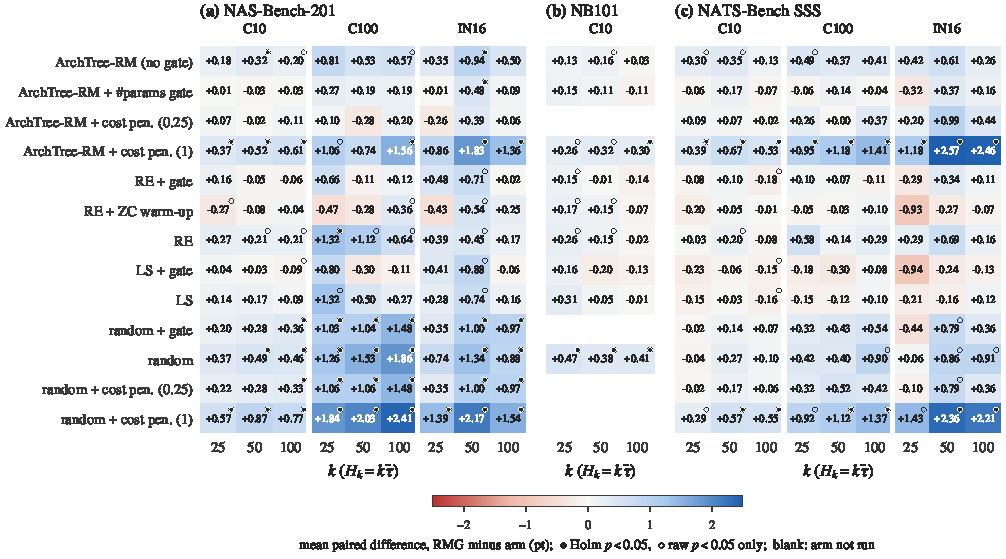
\includegraphics[width=\textwidth]{figs/figS5_egh_tests.pdf}
\caption{Mean paired difference in test accuracy between \rmg{} and every other arm at equal GPU-hours (blue: \rmg{} better), per dataset and budget multiple $k$. Filled dots: significant after Holm correction; open dots: $p<0.05$ before correction only.}
\label{f:egh}
\end{figure}

%% =====================================================================
\section{Rank-based statistics}\label{s:stats}

Table~\ref{t:friedman} reports the Friedman test for each of the five comparison sets, Tables~\ref{t:ranksfixed} and~\ref{t:ranksegh} all average ranks, Tables~\ref{t:pifixed} and~\ref{t:piegh} the probability that \rmg{} finds a better architecture on a paired run, and Table~\ref{t:tost} the equivalence tests. Equal performance of all methods is rejected everywhere ($p\le2.2\times10^{-8}$). \rmg{} has the best average rank on NAS-Bench-201 at equal GPU-hours and lies inside the critical difference of the top method in the other four sets. The per-run probabilities separate the field more finely than the ranks: in paired runs \rmg{} comes out ahead 75--85\% of the time against MCTS-style, random and ENAS-style search and LLM-NAS, 0.50--0.57 against RE, ZiCo-style and RZ-style search, and 41--43\% against RE with ZC warm-up and local search; at equal GPU-hours local search with the gate wins more paired runs on NAS-Bench-101 (0.22) and NATS-Bench SSS (0.38), as is RE with ZC warm-up on NATS-Bench SSS (0.40). Equivalence within $\pm$0.5\,pt is shown in at most 5 of 12 NAS-Bench-201 cells for any baseline and within $\pm$0.25\,pt in at most 3, so the ties in the Wilcoxon tests should be read as ``no detectable difference'', not as equality.

\begin{table}[tbp]
\caption{Friedman test per comparison set (blocks = dataset $\times$ budget $\times$ seed) with the Nemenyi critical difference (CD), the average rank of \rmg{} and the best method.}\label{t:friedman}
\centering\footnotesize
\setlength{\tabcolsep}{4pt}
\begin{tabular}{@{}lrrrrrrl@{}}
\toprule
Comparison & methods & blocks & $\chi^2_F$ & $p$ & CD & rank of RMG & best method (rank)\\
\midrule
NB201, fixed proposal budget & 10 & 144 & 381.2 & $1.4\times10^{-76}$ & 1.13 & 4.41 & RE + ZC warm-up (3.67)\\
NB201, equal GPU-hours & 14 & 108 & 428.1 & $2.5\times10^{-83}$ & 1.91 & 4.75 & ArchTree-RMG (4.75)\\
NB101, fixed proposal budget & 3 & 48 & 35.3 & $2.2\times10^{-8}$ & 0.48 & 1.73 & RE (1.58)\\
NB101, equal GPU-hours & 10 & 36 & 86.6 & $8.0\times10^{-15}$ & 2.26 & 4.38 & LS + gate (3.11)\\
NATS-SSS, equal GPU-hours & 14 & 108 & 416.9 & $6.0\times10^{-81}$ & 1.91 & 5.99 & LS + gate (4.19)\\
\bottomrule
\end{tabular}

\end{table}

\begin{table}[tbp]
\caption{Average Friedman rank at a fixed proposal budget (1 = best). $^{*}$: outside the CD of \rmg.}\label{t:ranksfixed}
\centering\footnotesize
\begin{tabular}{@{}lcc@{}}
\toprule
Method & NB201, fixed proposal budget & NB101, fixed proposal budget\\
\midrule
RE + ZC warm-up & 3.67 & --\\
Local search & 3.90 & --\\
\textbf{ArchTree-RMG} & \textbf{4.41} & \textbf{1.73}\\
RZ-style ZC walk & 4.41 & --\\
ZiCo-style & 4.47 & --\\
RE & 5.07 & 1.58\\
ENAS-style & 6.57$^{*}$ & --\\
LLM-NAS & 6.70$^{*}$ & --\\
Random search & 7.85$^{*}$ & --\\
MCTS-style & 7.97$^{*}$ & --\\
Random & -- & 2.69$^{*}$\\
\bottomrule
\end{tabular}

\end{table}

\begin{table}[tbp]
\caption{Average Friedman rank at equal GPU-hours (1 = best). $^{*}$: outside the CD of \rmg.}\label{t:ranksegh}
\centering\footnotesize
\begin{tabular}{@{}lccc@{}}
\toprule
Method & NB201, equal GPU-hours & NB101, equal GPU-hours & NATS-SSS, equal GPU-hours\\
\midrule
\textbf{ArchTree-RMG} & \textbf{4.75} & \textbf{4.38} & \textbf{5.99}\\
RE + ZC warm-up & 4.84 & 5.11 & 5.45\\
ArchTree-RM + cost pen. ($\lambda$=0.25) & 5.36 & -- & 7.42\\
ArchTree-RM + \#params gate & 5.47 & 5.08 & 6.15\\
LS + gate & 5.50 & 3.11 & 4.19\\
RE + gate & 6.03 & 4.56 & 6.01\\
LS & 6.91$^{*}$ & 5.03 & 5.55\\
RE & 8.04$^{*}$ & 5.81 & 7.46\\
ArchTree-RM (no gate) & 8.16$^{*}$ & 5.88 & 8.74$^{*}$\\
Random + gate & 9.07$^{*}$ & -- & 7.80\\
Random + cost pen. ($\lambda$=0.25) & 9.15$^{*}$ & -- & 7.94$^{*}$\\
ArchTree-RM + cost pen. ($\lambda$=1) & 9.58$^{*}$ & 7.57$^{*}$ & 11.93$^{*}$\\
Random & 10.20$^{*}$ & 8.49$^{*}$ & 8.66$^{*}$\\
Random + cost pen. ($\lambda$=1) & 11.94$^{*}$ & -- & 11.74$^{*}$\\
\bottomrule
\end{tabular}

\end{table}

\begin{table}[tbp]
\caption{Probability that \rmg{} finds a better architecture than the comparator on a paired (cell, seed) run at a fixed proposal budget, with stratified-bootstrap 95\% interval. Bold: interval above 0.5; italic: interval below 0.5.}\label{t:pifixed}
\centering\footnotesize
\begin{tabular}{@{}lcc@{}}
\toprule
Comparator & NB201, fixed proposal budget & NB101, fixed proposal budget\\
\midrule
RE + ZC warm-up & \textit{0.41 [0.34, 0.48]} & --\\
Local search & \textit{0.43 [0.36, 0.49]} & --\\
RZ-style ZC walk & 0.50 [0.42, 0.57] & --\\
ZiCo-style & 0.51 [0.44, 0.58] & --\\
RE & 0.57 [0.50, 0.64] & 0.44 [0.30, 0.57]\\
LLM-NAS & \textbf{0.75 [0.69, 0.81]} & --\\
ENAS-style & \textbf{0.77 [0.70, 0.83]} & --\\
Random search & \textbf{0.81 [0.75, 0.88]} & --\\
MCTS-style & \textbf{0.85 [0.79, 0.90]} & --\\
Random & -- & \textbf{0.83 [0.73, 0.94]}\\
\midrule
Paired runs & $n$ = 144 & $n$ = 48\\
\bottomrule
\end{tabular}

\end{table}

\begin{table}[tbp]
\caption{Probability that \rmg{} finds a better architecture at equal GPU-hours (layout as Table~\ref{t:pifixed}).}\label{t:piegh}
\centering\footnotesize
\begin{tabular}{@{}lccc@{}}
\toprule
Comparator & NB201, equal GPU-hours & NB101, equal GPU-hours & NATS-SSS, equal GPU-hours\\
\midrule
LS + gate & 0.50 [0.42, 0.58] & \textit{0.22 [0.08, 0.36]} & \textit{0.38 [0.29, 0.46]}\\
RE + ZC warm-up & 0.51 [0.43, 0.59] & 0.58 [0.42, 0.72] & \textit{0.40 [0.32, 0.49]}\\
ArchTree-RM + cost pen. ($\lambda$=0.25) & 0.53 [0.45, 0.60] & -- & 0.57 [0.49, 0.65]\\
ArchTree-RM + \#params gate & 0.56 [0.49, 0.64] & 0.58 [0.44, 0.72] & 0.49 [0.41, 0.58]\\
RE + gate & \textbf{0.60 [0.52, 0.69]} & 0.50 [0.35, 0.65] & 0.51 [0.43, 0.60]\\
LS & \textbf{0.61 [0.52, 0.69]} & \textbf{0.67 [0.51, 0.81]} & 0.47 [0.38, 0.56]\\
ArchTree-RM (no gate) & \textbf{0.76 [0.69, 0.83]} & \textbf{0.72 [0.58, 0.86]} & \textbf{0.69 [0.61, 0.76]}\\
RE & \textbf{0.79 [0.72, 0.86]} & 0.62 [0.49, 0.75] & \textbf{0.62 [0.54, 0.72]}\\
ArchTree-RM + cost pen. ($\lambda$=1) & \textbf{0.85 [0.79, 0.90]} & \textbf{0.81 [0.67, 0.92]} & \textbf{0.89 [0.84, 0.94]}\\
Random + cost pen. ($\lambda$=0.25) & \textbf{0.85 [0.79, 0.91]} & -- & \textbf{0.69 [0.60, 0.77]}\\
Random + gate & \textbf{0.85 [0.79, 0.91]} & -- & \textbf{0.67 [0.58, 0.75]}\\
Random & \textbf{0.90 [0.84, 0.94]} & \textbf{0.92 [0.81, 1.00]} & \textbf{0.72 [0.64, 0.80]}\\
Random + cost pen. ($\lambda$=1) & \textbf{0.94 [0.89, 0.97]} & -- & \textbf{0.91 [0.85, 0.95]}\\
\midrule
Paired runs & $n$ = 108 & $n$ = 36 & $n$ = 108\\
\bottomrule
\end{tabular}

\end{table}

\begin{table}[tbp]
\caption{Two one-sided tests (TOST, Holm-corrected): number of cells in which \rmg{} and the comparator are shown to be equivalent within $\pm$0.5 and $\pm$0.25\,pt, and the largest absolute mean difference over the cells.}\label{t:tost}
\centering\footnotesize
\begin{tabular}{@{}llrrrr@{}}
\toprule
Comparison & Comparator & cells & equiv. at $\pm$0.5 & equiv. at $\pm$0.25 & max $|\Delta|$\\
\midrule
NB201, fixed proposal budget & ENAS-style & 12 & 1 & 0 & 1.23\\
 & LLM-NAS & 12 & 3 & 1 & 1.27\\
 & Local search & 12 & 5 & 1 & 0.44\\
 & MCTS-style & 12 & 1 & 0 & 1.47\\
 & Random search & 12 & 0 & 0 & 1.48\\
 & RE & 12 & 4 & 2 & 1.08\\
 & RE + ZC warm-up & 12 & 5 & 1 & 0.83\\
 & RZ-style ZC walk & 12 & 5 & 3 & 0.25\\
 & ZiCo-style & 12 & 3 & 1 & 0.43\\
\midrule
NB201, equal GPU-hours & ArchTree-RM + cost pen. ($\lambda$=1) & 9 & 0 & 0 & 1.83\\
 & ArchTree-RM + cost pen. ($\lambda$=0.25) & 9 & 4 & 1 & 0.39\\
 & ArchTree-RM (no gate) & 9 & 2 & 0 & 0.94\\
 & ArchTree-RM + \#params gate & 9 & 3 & 1 & 0.48\\
 & LS & 9 & 1 & 0 & 1.32\\
 & LS + gate & 9 & 4 & 1 & 0.88\\
 & Random + cost pen. ($\lambda$=1) & 9 & 0 & 0 & 2.41\\
 & Random + cost pen. ($\lambda$=0.25) & 9 & 1 & 0 & 1.48\\
 & Random & 9 & 0 & 0 & 1.86\\
 & Random + gate & 9 & 0 & 0 & 1.48\\
 & RE & 9 & 2 & 0 & 1.32\\
 & RE + gate & 9 & 4 & 2 & 0.71\\
 & RE + ZC warm-up & 9 & 2 & 1 & 0.54\\
\midrule
NB101, fixed proposal budget & Random & 4 & 2 & 0 & 0.41\\
 & RE & 4 & 4 & 1 & 0.14\\
\midrule
NB101, equal GPU-hours & ArchTree-RM + cost pen. ($\lambda$=1) & 3 & 1 & 0 & 0.32\\
 & ArchTree-RM (no gate) & 3 & 3 & 1 & 0.16\\
 & ArchTree-RM + \#params gate & 3 & 3 & 0 & 0.15\\
 & LS & 3 & 2 & 1 & 0.31\\
 & LS + gate & 3 & 2 & 0 & 0.20\\
 & Random & 3 & 0 & 0 & 0.47\\
 & RE & 3 & 3 & 1 & 0.26\\
 & RE + gate & 3 & 3 & 1 & 0.15\\
 & RE + ZC warm-up & 3 & 3 & 0 & 0.17\\
\midrule
NATS-SSS, equal GPU-hours & ArchTree-RM + cost pen. ($\lambda$=1) & 9 & 0 & 0 & 2.57\\
 & ArchTree-RM + cost pen. ($\lambda$=0.25) & 9 & 3 & 1 & 0.99\\
 & ArchTree-RM (no gate) & 9 & 1 & 0 & 0.61\\
 & ArchTree-RM + \#params gate & 9 & 3 & 0 & 0.37\\
 & LS & 9 & 2 & 1 & 0.21\\
 & LS + gate & 9 & 2 & 1 & 0.94\\
 & Random + cost pen. ($\lambda$=1) & 9 & 0 & 0 & 2.36\\
 & Random + cost pen. ($\lambda$=0.25) & 9 & 3 & 0 & 0.79\\
 & Random & 9 & 2 & 0 & 0.91\\
 & Random + gate & 9 & 3 & 0 & 0.79\\
 & RE & 9 & 3 & 0 & 0.69\\
 & RE + gate & 9 & 3 & 0 & 0.34\\
 & RE + ZC warm-up & 9 & 3 & 2 & 0.93\\
\bottomrule
\end{tabular}

\end{table}

Figure~\ref{f:volcano} places the 749 accuracy comparisons of the main comparison families (listed in its panel b) on one plot; the sensitivity studies are excluded. The significant results lie almost entirely on the side favourable to \algname{} (154 of 155); the single loss is \algname-RM against RE, both with the parameter-count gate, on NAS-Bench-101 at a budget of 100 proposals.

\begin{figure}[tbp]
\centering
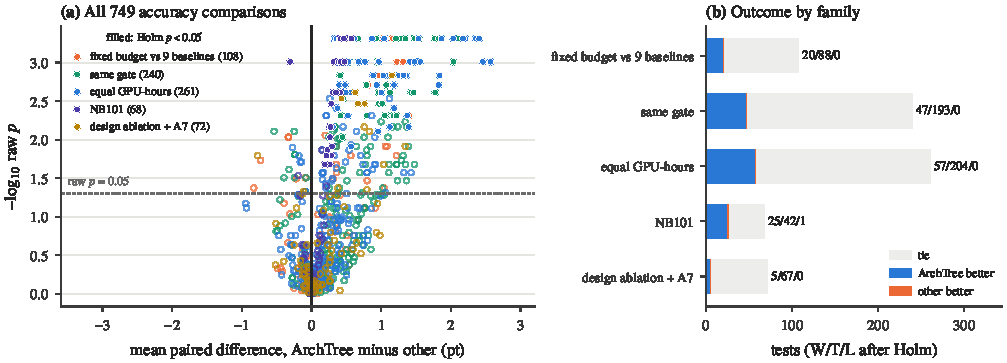
\includegraphics[width=\textwidth]{figs/figS15_volcano.pdf}
\caption{The 749 paired accuracy comparisons of \algname{} with another method or design variant in the five families of panel (b). (a) Mean paired difference against $-\log_{10}$ of the raw $p$-value; filled markers are significant after Holm correction (within baseline, arm or comparison, as in Table~8 of the main paper). The cap near $p\approx5\times10^{-4}$ is the smallest $p$-value an exact Wilcoxon test can give with 12 pairs. (b) Holm-corrected W/T/L per family.}
\label{f:volcano}
\end{figure}

%% =====================================================================
\section{The gate on every proposer}\label{s:grid}

Table~\ref{t:grid} gives all 24 proposer--gate combinations at a budget of 200 proposals, Figure~\ref{f:grid} the change in accuracy and the GPU-hours saved by each gate in every cell, and Table~\ref{t:gridtests} the comparison of \algname-RM with each other proposer under the same gate. At a fixed number of proposals, the label-free gate saves 25--72\% of GPU-hours across proposers, datasets and budgets. Its effect on accuracy depends on the proposer: it helps \algname-RM slightly (mean $+$0.11\,pt) and leaves random search unchanged, but costs MCTS-style search 0.36\,pt on average, because a proposer that generates few good candidates loses more when most of them are discarded. With the same gate, \algname-RM is never worse than any other proposer (W/T/L 7/5/0 against random, 9/3/0 against MCTS-style, 3/9/0 against ENAS-style search and 0/12/0 against RE and local search).

\begin{table}[tbp]
\caption{Proposer $\times$ gate grid on NAS-Bench-201 at a budget of 200 proposals: test accuracy (mean $\pm$ standard deviation), mean real evaluations, and GPU-hours summed over the three datasets.}\label{t:grid}
\centering\footnotesize
\setlength{\tabcolsep}{4pt}
\begin{tabular}{@{}llcrcrcrr@{}}
\toprule
\multirow{2}{*}{Proposer} & \multirow{2}{*}{Gate} & \multicolumn{2}{c}{CIFAR-10} & \multicolumn{2}{c}{CIFAR-100} & \multicolumn{2}{c}{ImageNet16-120} & GPU-h\\
\cmidrule(lr){3-4}\cmidrule(lr){5-6}\cmidrule(lr){7-8}
 & & acc. & evals & acc. & evals & acc. & evals & (3 sets)\\
\midrule
ArchTree-RM & none & 94.12 $\pm$ 0.24 & 200 & 72.97 $\pm$ 0.56 & 200 & 46.39 $\pm$ 0.45 & 200 & 1102\\
 & \#params & 94.32 $\pm$ 0.14 & 92 & 73.27 $\pm$ 0.31 & 97 & 46.27 $\pm$ 0.33 & 87 & 570\\
 & supervised & 94.26 $\pm$ 0.21 & 76 & 73.27 $\pm$ 0.23 & 79 & 46.43 $\pm$ 0.33 & 81 & 514\\
 & label-free & 94.28 $\pm$ 0.13 & 81 & 73.40 $\pm$ 0.20 & 82 & 46.41 $\pm$ 0.18 & 83 & 520\\
\midrule
RE & none & 94.31 $\pm$ 0.13 & 200 & 73.37 $\pm$ 0.21 & 200 & 46.48 $\pm$ 0.17 & 200 & 1162\\
 & \#params & 94.37 $\pm$ 0.00 & 116 & 73.34 $\pm$ 0.37 & 116 & 46.39 $\pm$ 0.51 & 112 & 716\\
 & supervised & 94.30 $\pm$ 0.14 & 93 & 73.51 $\pm$ 0.00 & 95 & 46.43 $\pm$ 0.18 & 106 & 649\\
 & label-free & 94.37 $\pm$ 0.00 & 105 & 73.44 $\pm$ 0.16 & 106 & 46.39 $\pm$ 0.20 & 103 & 652\\
\midrule
LS & none & 94.37 $\pm$ 0.00 & 200 & 73.51 $\pm$ 0.00 & 200 & 46.52 $\pm$ 0.29 & 200 & 1155\\
 & \#params & 94.37 $\pm$ 0.00 & 90 & 73.51 $\pm$ 0.00 & 94 & 46.37 $\pm$ 0.65 & 100 & 631\\
 & supervised & 94.31 $\pm$ 0.21 & 84 & 73.51 $\pm$ 0.00 & 81 & 46.16 $\pm$ 0.81 & 87 & 559\\
 & label-free & 94.37 $\pm$ 0.00 & 79 & 73.51 $\pm$ 0.00 & 83 & 46.51 $\pm$ 0.70 & 90 & 564\\
\midrule
Random & none & 93.92 $\pm$ 0.21 & 200 & 71.92 $\pm$ 0.81 & 200 & 45.47 $\pm$ 0.80 & 200 & 925\\
 & \#params & 93.90 $\pm$ 0.24 & 84 & 71.92 $\pm$ 0.82 & 84 & 45.48 $\pm$ 0.75 & 84 & 459\\
 & supervised & 93.92 $\pm$ 0.21 & 80 & 71.92 $\pm$ 0.81 & 79 & 45.47 $\pm$ 0.80 & 79 & 434\\
 & label-free & 93.92 $\pm$ 0.21 & 79 & 71.92 $\pm$ 0.81 & 79 & 45.47 $\pm$ 0.80 & 79 & 433\\
\midrule
ENAS-style & none & 94.09 $\pm$ 0.26 & 200 & 72.59 $\pm$ 0.81 & 200 & 46.16 $\pm$ 0.36 & 200 & 1068\\
 & \#params & 94.01 $\pm$ 0.22 & 84 & 72.25 $\pm$ 1.07 & 86 & 45.78 $\pm$ 0.69 & 81 & 494\\
 & supervised & 93.81 $\pm$ 0.33 & 78 & 72.49 $\pm$ 0.84 & 75 & 45.71 $\pm$ 0.93 & 74 & 453\\
 & label-free & 93.96 $\pm$ 0.22 & 77 & 72.41 $\pm$ 1.06 & 78 & 45.86 $\pm$ 0.74 & 74 & 455\\
\midrule
MCTS-style & none & 93.88 $\pm$ 0.19 & 200 & 71.76 $\pm$ 0.86 & 200 & 45.60 $\pm$ 0.64 & 200 & 938\\
 & \#params & 93.73 $\pm$ 0.32 & 67 & 71.43 $\pm$ 0.83 & 69 & 45.20 $\pm$ 0.90 & 76 & 380\\
 & supervised & 93.94 $\pm$ 0.18 & 61 & 71.45 $\pm$ 0.55 & 54 & 45.19 $\pm$ 0.73 & 52 & 272\\
 & label-free & 93.62 $\pm$ 0.42 & 56 & 71.29 $\pm$ 0.69 & 61 & 44.87 $\pm$ 0.82 & 54 & 276\\
\bottomrule
\end{tabular}

\end{table}

\begin{table}[tbp]
\caption{\algname-RM against each other proposer when both use the same gate: Holm-corrected W/T/L over 12 dataset--budget cells and mean paired difference (pt).}\label{t:gridtests}
\centering\footnotesize
\begin{tabular}{@{}lcccccccc@{}}
\toprule
\multirow{2}{*}{Other proposer} & \multicolumn{2}{c}{no gate} & \multicolumn{2}{c}{\#params} & \multicolumn{2}{c}{supervised} & \multicolumn{2}{c}{label-free}\\
\cmidrule(lr){2-3}\cmidrule(lr){4-5}\cmidrule(lr){6-7}\cmidrule(lr){8-9}
 & W/T/L & mean $\Delta$ & W/T/L & mean $\Delta$ & W/T/L & mean $\Delta$ & W/T/L & mean $\Delta$\\
\midrule
Random & 3/9/0 & 0.66 & 6/6/0 & 0.70 & 2/10/0 & 0.71 & 7/5/0 & 0.77\\
RE & 0/12/0 & 0.13 & 0/12/0 & 0.12 & 1/11/0 & 0.20 & 0/12/0 & 0.20\\
LS & 0/12/0 & $-$0.19 & 0/12/0 & $-$0.07 & 0/12/0 & 0.12 & 0/12/0 & 0.09\\
ENAS-style & 0/12/0 & 0.31 & 1/11/0 & 0.49 & 3/9/0 & 0.51 & 3/9/0 & 0.53\\
MCTS-style & 2/10/0 & 0.76 & 6/6/0 & 1.01 & 4/8/0 & 0.97 & 9/3/0 & 1.23\\
\bottomrule
\end{tabular}

\end{table}

\begin{figure}[tbp]
\centering
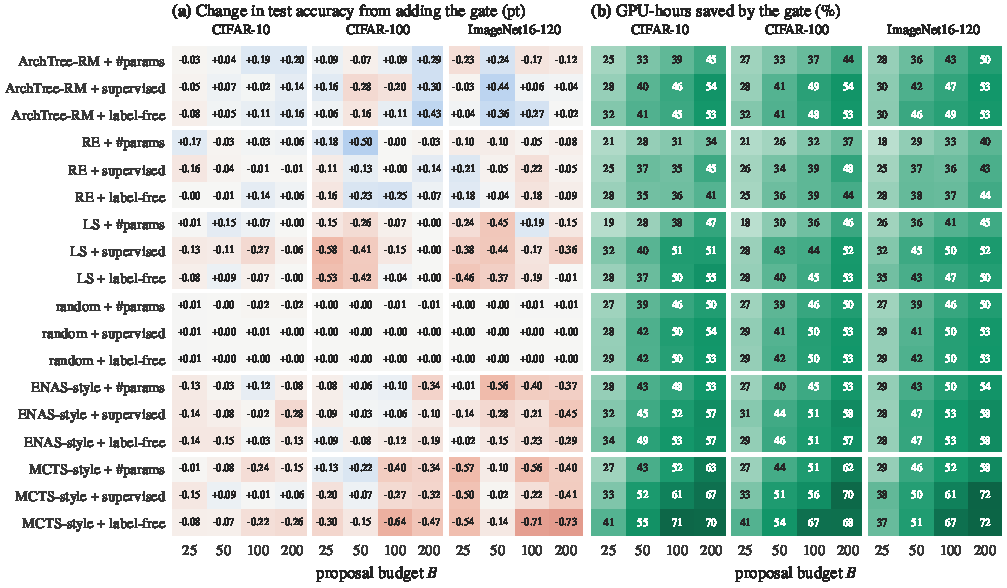
\includegraphics[width=\textwidth]{figs/figS6_gate_grid.pdf}
\caption{Effect of each gate on each proposer at a fixed number of proposals (NAS-Bench-201, 12 seeds). (a) Mean test accuracy with the gate minus without it. (b) Share of GPU-hours saved by the gate.}
\label{f:grid}
\end{figure}

%% =====================================================================
\section{Ablations and sensitivity}\label{s:abl}

\textit{Held-out design ablation.} Table~\ref{t:design} repeats the base$\to$RMG design changes on 12 seeds that were not consulted for any design choice. Only four of 48 comparisons are significant, all in favour of \rmg: the base system with the gate on all three datasets at 200 proposals, and the rank reward alone on ImageNet16-120. Mutation alone and RE with the same gate are statistically indistinguishable from \rmg{} at every budget; at 200 proposals RE is within 0.11\,pt of \rmg{} on every dataset but uses 99--105 real evaluations against 84--90.

\begin{table}[tbp]
\caption{Held-out design ablation (seeds 7--909): test accuracy (mean $\pm$ standard deviation) of each variant, all with the label-free gate, and real evaluations at $B$ = 200. $^{\triangledown}$: \rmg{} significantly better (Holm within arm over 12 cells, $p_{\mathrm{Holm}}<0.05$).}\label{t:design}
\centering\footnotesize
\begin{tabular}{@{}lccccr@{}}
\toprule
Arm & $B$ = 25 & $B$ = 50 & $B$ = 100 & $B$ = 200 & evals ($B$=200)\\
\midrule
\multicolumn{6}{@{}l}{\textit{CIFAR-10}}\\
\quad ArchTree-base + gate & 93.24 $\pm$ 0.60 & 93.46 $\pm$ 0.43 & 93.79 $\pm$ 0.38 & 93.83 $\pm$ 0.30$^{\triangledown}$ & 83.8\\
\quad rank reward only & 93.51 $\pm$ 0.56 & 93.88 $\pm$ 0.51 & 94.00 $\pm$ 0.28 & 94.17 $\pm$ 0.22 & 71.0\\
\quad mutation only & 93.62 $\pm$ 0.45 & 93.94 $\pm$ 0.37 & 94.23 $\pm$ 0.21 & 94.32 $\pm$ 0.14 & 93.7\\
\quad RE + same gate & 93.56 $\pm$ 0.53 & 94.03 $\pm$ 0.31 & 94.30 $\pm$ 0.18 & 94.37 $\pm$ 0.00 & 99.3\\
\quad ArchTree-RMG & 93.51 $\pm$ 0.44 & 93.81 $\pm$ 0.28 & 94.17 $\pm$ 0.23 & 94.26 $\pm$ 0.18 & 83.6\\
\midrule
\multicolumn{6}{@{}l}{\textit{CIFAR-100}}\\
\quad ArchTree-base + gate & 70.40 $\pm$ 1.20 & 70.93 $\pm$ 1.08 & 71.54 $\pm$ 1.05 & 72.27 $\pm$ 0.78$^{\triangledown}$ & 82.9\\
\quad rank reward only & 71.33 $\pm$ 1.06 & 71.98 $\pm$ 1.07 & 72.42 $\pm$ 0.96 & 72.59 $\pm$ 0.97 & 65.8\\
\quad mutation only & 71.09 $\pm$ 1.12 & 71.82 $\pm$ 1.17 & 72.98 $\pm$ 0.82 & 73.38 $\pm$ 0.27 & 92.9\\
\quad RE + same gate & 70.76 $\pm$ 1.09 & 72.06 $\pm$ 0.46 & 72.79 $\pm$ 0.92 & 73.37 $\pm$ 0.21 & 105.2\\
\quad ArchTree-RMG & 71.35 $\pm$ 0.86 & 71.97 $\pm$ 0.89 & 72.89 $\pm$ 0.76 & 73.42 $\pm$ 0.17 & 84.0\\
\midrule
\multicolumn{6}{@{}l}{\textit{ImageNet16-120}}\\
\quad ArchTree-base + gate & 44.17 $\pm$ 1.27 & 45.04 $\pm$ 1.12 & 45.35 $\pm$ 0.67 & 45.72 $\pm$ 0.50$^{\triangledown}$ & 82.8\\
\quad rank reward only & 44.63 $\pm$ 1.09 & 45.55 $\pm$ 0.68 & 45.39 $\pm$ 0.68 & 45.62 $\pm$ 0.60$^{\triangledown}$ & 71.0\\
\quad mutation only & 44.70 $\pm$ 0.92 & 45.31 $\pm$ 1.00 & 46.13 $\pm$ 0.63 & 46.14 $\pm$ 0.60 & 98.8\\
\quad RE + same gate & 45.11 $\pm$ 0.80 & 45.70 $\pm$ 0.82 & 46.39 $\pm$ 0.27 & 46.45 $\pm$ 0.19 & 101.5\\
\quad ArchTree-RMG & 44.59 $\pm$ 1.25 & 45.30 $\pm$ 0.92 & 45.62 $\pm$ 0.87 & 46.39 $\pm$ 0.27 & 90.4\\
\bottomrule
\end{tabular}

\end{table}

\textit{Trie against a flat bandit (A7).} Table~\ref{t:a7} compares the trie with a per-position UCB that either remembers evaluated architectures in a set or does not. With the set, no difference reaches $p<0.05$ (12 cells), so the hierarchy itself adds nothing measurable. Without it, the flat bandit spends 11.7--94.7 evaluations per run on repeats and is worse in three cells before correction and one after (ImageNet16-120, $B=100$).

\begin{table}[tbp]
\caption{Trie against a flat per-position UCB with and without set-based deduplication: test accuracy (mean $\pm$ standard deviation), mean unique and repeated real evaluations, and paired difference (pt) of the trie with the unadjusted Wilcoxon $p$-value.}\label{t:a7}
\centering\scriptsize
\setlength{\tabcolsep}{3pt}
\begin{tabular}{@{}lrcccccccc@{}}
\toprule
\multirow{2}{*}{Dataset} & \multirow{2}{*}{$B$} & \multicolumn{2}{c}{trie} & \multicolumn{2}{c}{flat UCB + set dedup} & \multicolumn{2}{c}{flat UCB, no dedup} & \multicolumn{2}{c}{trie minus ($p$)}\\
\cmidrule(lr){3-4}\cmidrule(lr){5-6}\cmidrule(lr){7-8}\cmidrule(lr){9-10}
 & & acc. & uniq./dup. & acc. & uniq./dup. & acc. & uniq./dup. & flat+set & flat\\
\midrule
CIFAR-10 & 25 & 93.60 $\pm$ 0.31 & 16.4 / 0.0 & 93.76 $\pm$ 0.40 & 16.5 / 0.0 & 93.27 $\pm$ 0.59 & 7.9 / 11.7 & $-$0.16 (0.375) & 0.33 (0.203)\\
 & 50 & 94.04 $\pm$ 0.27 & 27.1 / 0.0 & 94.14 $\pm$ 0.30 & 26.9 / 0.0 & 93.83 $\pm$ 0.47 & 13.2 / 22.6 & $-$0.10 (0.465) & 0.20 (0.465)\\
 & 100 & 94.19 $\pm$ 0.26 & 47.8 / 0.0 & 94.22 $\pm$ 0.21 & 47.8 / 0.0 & 94.14 $\pm$ 0.35 & 21.8 / 45.7 & $-$0.03 (0.676) & 0.05 (0.910)\\
 & 200 & 94.28 $\pm$ 0.13 & 80.8 / 0.0 & 94.32 $\pm$ 0.13 & 83.9 / 0.0 & 94.22 $\pm$ 0.35 & 34.6 / 94.2 & $-$0.04 (0.469) & 0.06 (0.812)\\
\midrule
CIFAR-100 & 25 & 71.51 $\pm$ 1.26 & 16.4 / 0.0 & 71.10 $\pm$ 1.17 & 17.2 / 0.0 & 70.53 $\pm$ 1.28 & 7.7 / 11.8 & 0.41 (0.910) & 0.98 (0.175)\\
 & 50 & 72.19 $\pm$ 0.91 & 27.2 / 0.0 & 72.38 $\pm$ 1.10 & 26.8 / 0.0 & 71.48 $\pm$ 1.53 & 12.7 / 22.2 & $-$0.19 (0.470) & 0.71 (0.301)\\
 & 100 & 73.02 $\pm$ 0.75 & 47.1 / 0.0 & 72.76 $\pm$ 0.90 & 48.0 / 0.0 & 72.23 $\pm$ 1.14 & 21.5 / 46.6 & 0.26 (0.391) & 0.79 (0.045)\\
 & 200 & 73.40 $\pm$ 0.20 & 81.5 / 0.0 & 73.14 $\pm$ 0.37 & 86.2 / 0.0 & 72.76 $\pm$ 1.15 & 32.8 / 94.1 & 0.26 (0.055) & 0.65 (0.219)\\
\midrule
ImageNet16-120 & 25 & 45.28 $\pm$ 1.07 & 16.5 / 0.0 & 45.13 $\pm$ 1.19 & 17.5 / 0.0 & 44.35 $\pm$ 1.67 & 7.8 / 11.8 & 0.15 (0.770) & 0.93 (0.160)\\
 & 50 & 45.91 $\pm$ 0.51 & 24.8 / 0.0 & 45.80 $\pm$ 1.14 & 26.7 / 0.0 & 45.16 $\pm$ 0.78 & 12.6 / 24.1 & 0.12 (0.910) & 0.76 (0.007)\\
 & 100 & 46.45 $\pm$ 0.39 & 45.4 / 0.0 & 46.33 $\pm$ 0.77 & 47.2 / 0.0 & 45.83 $\pm$ 0.63 & 21.4 / 48.2 & 0.13 (0.557) & 0.63 (0.002)\\
 & 200 & 46.41 $\pm$ 0.18 & 82.8 / 0.0 & 46.45 $\pm$ 0.42 & 83.3 / 0.0 & 46.12 $\pm$ 0.65 & 33.0 / 94.7 & $-$0.04 (0.676) & 0.29 (0.276)\\
\bottomrule
\end{tabular}

\end{table}

\textit{Toggle ablations (A1--A6).} Table~\ref{t:toggles} shows that removing the LLM prior (A1), weight inheritance (A3) or rerunning the budget grid (A6) reproduces the headline runs exactly (144 of 144 runs each, same accuracy and same number of evaluations), as expected with $\alpha=0$ and tabular benchmarks; these rows document that the components are inert, not that they were tested for an effect. Removing the gate (A2) uses every proposal and changes the mean by $-$0.43 to $+$0.16\,pt. Table~\ref{t:a5} varies the share of pruned nodes: between 0 and 35\% the mean accuracy moves by less than 0.2\,pt, except a drop of 0.41\,pt on ImageNet16-120 at 35\%, which is consistent with the moderate default of 15\%.

\begin{table}[tbp]
\caption{Toggle ablations on NAS-Bench-201: mean test accuracy and, in brackets, mean real evaluations.}\label{t:toggles}
\centering\footnotesize
\begin{tabular}{@{}lrccccc@{}}
\toprule
Dataset & $B$ & S4 \rmg{} & A1 no LLM & A2 no gate & A3 no inheritance & A6 budget grid\\
\midrule
CIFAR-10 & 25 & 93.60 (16.4) & 93.60 (16.4) & 93.68 (25.0) & 93.60 (16.4) & 93.60 (16.4)\\
 & 50 & 94.04 (27.1) & 94.04 (27.1) & 93.99 (50.0) & 94.04 (27.1) & 94.04 (27.1)\\
 & 100 & 94.19 (47.8) & 94.19 (47.8) & 94.07 (100.0) & 94.19 (47.8) & 94.19 (47.8)\\
 & 200 & 94.28 (80.8) & 94.28 (80.8) & 94.12 (200.0) & 94.28 (80.8) & 94.28 (80.8)\\
\midrule
CIFAR-100 & 25 & 71.51 (16.4) & 71.51 (16.4) & 71.45 (25.0) & 71.51 (16.4) & 71.51 (16.4)\\
 & 50 & 72.19 (27.2) & 72.19 (27.2) & 72.35 (50.0) & 72.19 (27.2) & 72.19 (27.2)\\
 & 100 & 73.02 (47.1) & 73.02 (47.1) & 72.91 (100.0) & 73.02 (47.1) & 73.02 (47.1)\\
 & 200 & 73.40 (81.5) & 73.40 (81.5) & 72.97 (200.0) & 73.40 (81.5) & 73.40 (81.5)\\
\midrule
ImageNet16-120 & 25 & 45.28 (16.5) & 45.28 (16.5) & 45.24 (25.0) & 45.28 (16.5) & 45.28 (16.5)\\
 & 50 & 45.91 (24.8) & 45.91 (24.8) & 45.56 (50.0) & 45.91 (24.8) & 45.91 (24.8)\\
 & 100 & 46.45 (45.4) & 46.45 (45.4) & 46.18 (100.0) & 46.45 (45.4) & 46.45 (45.4)\\
 & 200 & 46.41 (82.8) & 46.41 (82.8) & 46.39 (200.0) & 46.41 (82.8) & 46.41 (82.8)\\
\bottomrule
\end{tabular}

\end{table}

\begin{table}[tbp]
\caption{Pruning share (A5) at $B$ = 100: test accuracy (mean $\pm$ standard deviation) and mean real evaluations.}\label{t:a5}
\centering\footnotesize
\begin{tabular}{@{}lccc@{}}
\toprule
Pruned share & CIFAR-10 & CIFAR-100 & ImageNet16-120\\
\midrule
0\% & 94.19 $\pm$ 0.26 (47.6) & 73.16 $\pm$ 0.33 (48.1) & 46.36 $\pm$ 0.50 (45.9)\\
15\% (default) & 94.19 $\pm$ 0.26 (47.8) & 73.02 $\pm$ 0.75 (47.1) & 46.45 $\pm$ 0.39 (45.4)\\
25\% & 94.22 $\pm$ 0.22 (47.5) & 73.04 $\pm$ 0.59 (46.8) & 46.34 $\pm$ 0.55 (46.6)\\
35\% & 94.22 $\pm$ 0.20 (47.2) & 73.19 $\pm$ 0.36 (47.0) & 46.04 $\pm$ 0.60 (46.4)\\
\bottomrule
\end{tabular}

\end{table}

\textit{UCB constant and backup.} Table~\ref{t:ucb} and Figure~\ref{f:ucb} vary $C$ from 0.1 to 2 under both backup rules. None of the 78 comparisons with the default is significant after correction (9 before). Large constants make the descent close to uniform over children (no duplicate proposals for $C\ge\sqrt2$), whereas small constants repeat good branches and lean more on deduplication; the max backup is the more robust rule, particularly on CIFAR-100, where the mean backup loses up to 0.75\,pt.

\begin{table}[tbp]
\caption{UCB sensitivity: mean test accuracy for each exploration constant $C$ and backup rule at $B$ = 100 and 200, and mean number of proposals redirected because they were duplicates. Bold: default.}\label{t:ucb}
\centering\footnotesize
\begin{tabular}{@{}llrrrrrrr@{}}
\toprule
\multirow{2}{*}{Backup} & \multirow{2}{*}{$C$} & \multicolumn{2}{c}{CIFAR-10} & \multicolumn{2}{c}{CIFAR-100} & \multicolumn{2}{c}{ImageNet16-120} & dup.\\
\cmidrule(lr){3-4}\cmidrule(lr){5-6}\cmidrule(lr){7-8}
 & & 100 & 200 & 100 & 200 & 100 & 200 & proposals\\
\midrule
mean & 0.1 & 94.28 & 94.32 & 72.88 & 73.09 & 46.17 & 46.32 & 29.6\\
 & 0.2 & 94.25 & 94.33 & 72.62 & 73.03 & 46.47 & 46.28 & 23.6\\
 & 0.3 & 94.10 & 94.24 & 72.93 & 73.13 & 46.28 & 46.44 & 14.7\\
 & 0.5 & 94.16 & 94.24 & 72.52 & 72.84 & 45.99 & 46.37 & 8.5\\
 & 1 & 93.98 & 94.20 & 72.49 & 73.06 & 46.09 & 46.41 & 0.3\\
 & $\sqrt{2}$ & 94.13 & 94.24 & 72.27 & 73.02 & 46.13 & 46.36 & 0.0\\
 & 2 & 94.14 & 94.23 & 72.27 & 72.97 & 45.91 & 46.37 & 0.0\\
\midrule
max & 0.1 & 94.19 & 94.25 & 72.90 & 73.27 & 46.19 & 46.42 & 36.6\\
 & 0.2 & 94.16 & 94.24 & 72.87 & 73.36 & 46.45 & 46.54 & 27.7\\
 & 0.3 & \textbf{94.19} & \textbf{94.28} & \textbf{73.02} & \textbf{73.40} & \textbf{46.45} & \textbf{46.41} & 17.4\\
 & 0.5 & 94.16 & 94.28 & 72.98 & 73.33 & 46.37 & 46.45 & 10.7\\
 & 1 & 94.15 & 94.18 & 72.94 & 73.32 & 45.98 & 46.57 & 0.2\\
 & $\sqrt{2}$ & 94.11 & 94.13 & 72.54 & 73.13 & 46.21 & 46.14 & 0.0\\
 & 2 & 94.02 & 94.30 & 72.68 & 73.21 & 46.16 & 46.19 & 0.0\\
\bottomrule
\end{tabular}

\end{table}

\begin{figure}[tbp]
\centering
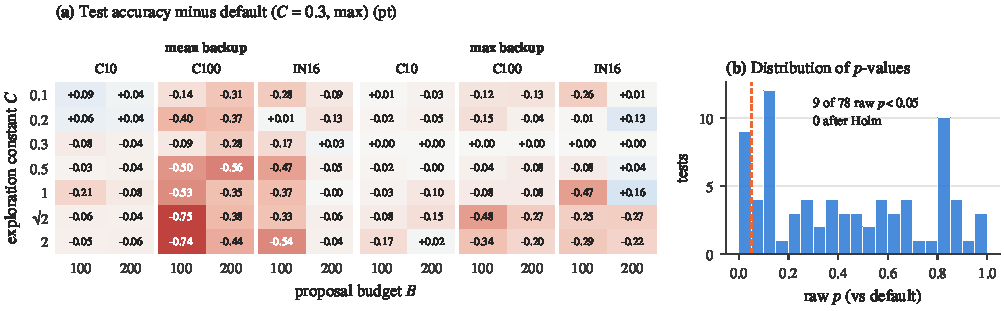
\includegraphics[width=\textwidth]{figs/figS7_ucb.pdf}
\caption{UCB sensitivity. (a) Test accuracy relative to the default ($C$ = 0.3, max backup) for every $C$, backup rule, dataset and budget. (b) Distribution of the 78 unadjusted $p$-values against the default.}
\label{f:ucb}
\end{figure}

\textit{Proxy subsets.} Table~\ref{t:subsets} and Figure~\ref{f:subsets} run the search with every subset of the four proxies as gate. The ranking quality of a subset predicts search accuracy only on ImageNet16-120 (Spearman 0.54, $p$ = 0.04; CIFAR-10 0.02, CIFAR-100 0.15). SVD entropy alone is the only subset that is significantly worse than the four-proxy combination (CIFAR-10 $-$0.45\,pt and CIFAR-100 $-$1.11\,pt; the only 2 of 48 comparisons significant after correction); all other subsets lie within the seed-to-seed spread of each other. In this ablation each subset is combined with weights fitted on the calibration architectures, so it isolates the choice of proxies; the $EST$ subset reaches $\tau$ = 0.66, 0.71 and 0.62, within 0.04 of the best subset on every dataset, and the label-free equal-weight version used in the paper ranks almost as well (Table~\ref{t:calib}).

\begin{table}[tbp]
\caption{Proxy subsets as gate ($B$ = 100): Kendall $\tau$ of the subset score with validation accuracy, test accuracy (mean $\pm$ standard deviation) and mean real evaluations. Subsets are combined with fitted weights.}\label{t:subsets}
\centering\scriptsize
\setlength{\tabcolsep}{3.5pt}
\begin{tabular}{@{}lrcrrcrrcr@{}}
\toprule
\multirow{2}{*}{Proxies} & \multicolumn{3}{c}{CIFAR-10} & \multicolumn{3}{c}{CIFAR-100} & \multicolumn{3}{c}{ImageNet16-120}\\
\cmidrule(lr){2-4}\cmidrule(lr){5-7}\cmidrule(lr){8-10}
 & $\tau$ & acc. & evals & $\tau$ & acc. & evals & $\tau$ & acc. & evals\\
\midrule
$E$ & 0.54 & 93.65 $\pm$ 0.35 & 42.7 & 0.52 & 71.59 $\pm$ 1.18 & 44.6 & 0.48 & 45.83 $\pm$ 0.43 & 47.4\\
$S$ & 0.54 & 94.24 $\pm$ 0.20 & 48.2 & 0.57 & 73.04 $\pm$ 0.57 & 48.2 & 0.55 & 46.22 $\pm$ 0.56 & 47.4\\
$T$ & 0.59 & 94.19 $\pm$ 0.26 & 47.2 & 0.62 & 72.89 $\pm$ 0.71 & 46.9 & 0.58 & 46.30 $\pm$ 0.51 & 44.0\\
$C$ & 0.48 & 94.26 $\pm$ 0.20 & 50.5 & 0.49 & 72.64 $\pm$ 0.78 & 50.8 & 0.46 & 46.18 $\pm$ 0.59 & 47.6\\
$ES$ & 0.70 & 94.05 $\pm$ 0.22 & 43.5 & 0.70 & 72.66 $\pm$ 1.01 & 45.8 & 0.61 & 46.46 $\pm$ 0.40 & 46.2\\
$ET$ & 0.59 & 93.76 $\pm$ 0.32 & 42.0 & 0.62 & 71.95 $\pm$ 1.29 & 41.8 & 0.60 & 46.23 $\pm$ 0.44 & 45.9\\
$EC$ & 0.66 & 94.18 $\pm$ 0.28 & 45.2 & 0.65 & 72.74 $\pm$ 1.22 & 47.9 & 0.57 & 46.37 $\pm$ 0.57 & 44.7\\
$ST$ & 0.56 & 94.16 $\pm$ 0.21 & 47.8 & 0.59 & 72.86 $\pm$ 0.80 & 47.6 & 0.56 & 46.19 $\pm$ 0.66 & 47.2\\
$SC$ & 0.50 & 94.09 $\pm$ 0.26 & 47.8 & 0.56 & 72.92 $\pm$ 0.57 & 46.5 & 0.55 & 46.14 $\pm$ 0.58 & 46.8\\
$TC$ & 0.57 & 94.24 $\pm$ 0.18 & 46.8 & 0.57 & 72.64 $\pm$ 0.95 & 47.9 & 0.52 & 46.50 $\pm$ 0.46 & 46.1\\
$EST$ & 0.66 & 94.18 $\pm$ 0.35 & 44.5 & 0.71 & 72.90 $\pm$ 0.77 & 46.7 & 0.62 & 46.47 $\pm$ 0.39 & 47.1\\
$ESC$ & 0.69 & 94.27 $\pm$ 0.14 & 46.2 & 0.70 & 72.80 $\pm$ 0.85 & 46.7 & 0.62 & 46.27 $\pm$ 0.57 & 47.1\\
$ETC$ & 0.65 & 94.02 $\pm$ 0.35 & 44.9 & 0.67 & 72.69 $\pm$ 0.95 & 48.1 & 0.60 & 46.44 $\pm$ 0.68 & 44.2\\
$STC$ & 0.50 & 94.08 $\pm$ 0.28 & 46.9 & 0.58 & 73.06 $\pm$ 0.55 & 47.2 & 0.56 & 46.19 $\pm$ 0.66 & 47.2\\
$ESTC$ & 0.66 & 94.10 $\pm$ 0.30 & 46.1 & 0.70 & 72.70 $\pm$ 0.92 & 45.7 & 0.63 & 46.24 $\pm$ 0.63 & 46.8\\
no gate & -- & 94.07 $\pm$ 0.27 & 100.0 & -- & 72.91 $\pm$ 0.59 & 100.0 & -- & 46.18 $\pm$ 0.41 & 100.0\\
\bottomrule
\end{tabular}

\end{table}

\begin{figure}[tbp]
\centering
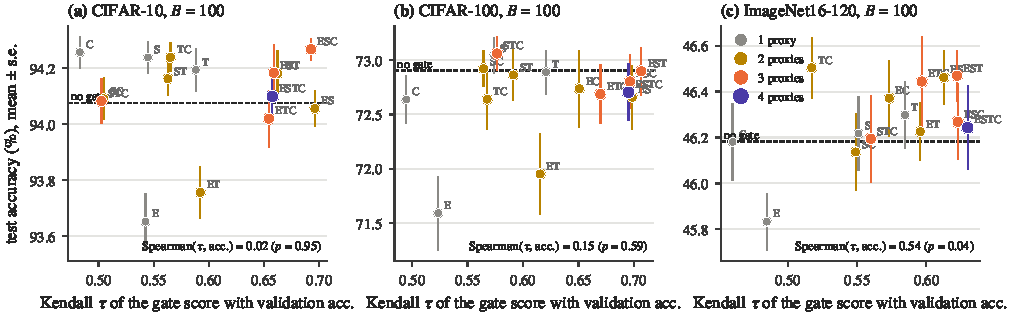
\includegraphics[width=\textwidth]{figs/figS8_proxy_subsets.pdf}
\caption{Ranking quality of each proxy subset against the accuracy reached with it as gate (mean $\pm$ standard error; colour and size: number of proxies). The dashed line is the search without a gate.}
\label{f:subsets}
\end{figure}

%% =====================================================================
\section{NAS-Bench-101}\label{s:nb101}

Table~\ref{t:nb101} gives every proposer--gate--budget cell on NAS-Bench-101, Table~\ref{t:nb101tests} the comparisons under the same gate and Table~\ref{t:nb101matched} the comparisons with ungated searches that receive at least as many real evaluations (11 wins, all against random search or the ungated \algname-RM); Figure~\ref{f:nb101} plots them. \algname-RM beats random search in 14 of 16 cells and ties RE in 15, the exception being a loss to RE with the parameter-count gate at 100 proposals. The gates leave 39--55\% of the real evaluations of \algname-RM (for example 162.8 instead of 400 with the label-free gate) without a consistent loss of accuracy, although the gain is smaller than on NAS-Bench-201 because the proxies rank NAS-Bench-101 less well (Table~\ref{t:calib}).

\begin{table}[tbp]
\caption{NAS-Bench-101 (CIFAR-10): test accuracy (mean $\pm$ standard deviation) and, in brackets, mean real evaluations for each proposer, gate and proposal budget $B$.}\label{t:nb101}
\centering\scriptsize
\setlength{\tabcolsep}{4pt}
\begin{tabular}{@{}llcccc@{}}
\toprule
Proposer & Gate & $B$ = 50 & $B$ = 100 & $B$ = 200 & $B$ = 400\\
\midrule
ArchTree-RM & none & 93.51 $\pm$ 0.22 (50) & 93.71 $\pm$ 0.23 (100) & 93.81 $\pm$ 0.24 (200) & 93.94 $\pm$ 0.20 (400)\\
 & \#params & 93.51 $\pm$ 0.24 (27) & 93.60 $\pm$ 0.14 (47) & 93.98 $\pm$ 0.19 (85) & 93.91 $\pm$ 0.21 (163)\\
 & supervised & 93.54 $\pm$ 0.30 (26) & 93.69 $\pm$ 0.25 (45) & 93.88 $\pm$ 0.24 (82) & 93.96 $\pm$ 0.24 (158)\\
 & label-free & 93.60 $\pm$ 0.19 (28) & 93.76 $\pm$ 0.18 (48) & 93.82 $\pm$ 0.18 (89) & 93.96 $\pm$ 0.19 (163)\\
\midrule
RE & none & 93.53 $\pm$ 0.21 (50) & 93.76 $\pm$ 0.26 (100) & 93.92 $\pm$ 0.25 (200) & 94.13 $\pm$ 0.12 (400)\\
 & \#params & 93.55 $\pm$ 0.24 (26) & 93.90 $\pm$ 0.19 (48) & 93.98 $\pm$ 0.18 (90) & 94.07 $\pm$ 0.15 (164)\\
 & supervised & 93.50 $\pm$ 0.28 (25) & 93.73 $\pm$ 0.21 (44) & 93.98 $\pm$ 0.21 (84) & 94.05 $\pm$ 0.19 (155)\\
 & label-free & 93.50 $\pm$ 0.23 (27) & 93.78 $\pm$ 0.25 (44) & 93.96 $\pm$ 0.24 (82) & 94.07 $\pm$ 0.20 (154)\\
\midrule
Random & none & 93.38 $\pm$ 0.16 (50) & 93.41 $\pm$ 0.20 (100) & 93.49 $\pm$ 0.13 (200) & 93.68 $\pm$ 0.12 (400)\\
 & \#params & 93.33 $\pm$ 0.22 (27) & 93.41 $\pm$ 0.20 (44) & 93.49 $\pm$ 0.13 (79) & 93.68 $\pm$ 0.12 (150)\\
 & supervised & 93.28 $\pm$ 0.26 (26) & 93.39 $\pm$ 0.20 (43) & 93.47 $\pm$ 0.18 (81) & 93.68 $\pm$ 0.12 (150)\\
 & label-free & 93.34 $\pm$ 0.22 (28) & 93.35 $\pm$ 0.23 (43) & 93.44 $\pm$ 0.15 (78) & 93.68 $\pm$ 0.12 (147)\\
\bottomrule
\end{tabular}

\end{table}

\begin{table}[tbp]
\caption{NAS-Bench-101: \algname-RM against random search and RE under the same gate (W/T/L over four budgets, mean paired difference in pt).}\label{t:nb101tests}
\centering\footnotesize
\setlength{\tabcolsep}{3pt}
\begin{tabular}{@{}lcccc@{}}
\toprule
\multirow{2}{*}{Gate (same for both)} & \multicolumn{2}{c}{ArchTree-RM vs random} & \multicolumn{2}{c}{ArchTree-RM vs RE}\\
\cmidrule(lr){2-3}\cmidrule(lr){4-5}
 & W/T/L & mean $\Delta$ & W/T/L & mean $\Delta$\\
\midrule
none & 3/1/0 & 0.250 & 0/4/0 & $-$0.096\\
\#params & 3/1/0 & 0.270 & 0/3/1 & $-$0.127\\
supervised & 4/0/0 & 0.308 & 0/4/0 & $-$0.047\\
label-free & 4/0/0 & 0.334 & 0/4/0 & $-$0.044\\
\bottomrule
\end{tabular}

\end{table}

\begin{table}[tbp]
\caption{NAS-Bench-101 with matched evaluations: gated \algname-RM at proposal budget $B$ against ungated random search, RE and \algname-RM given the smallest budget at least as large as the gated run's maximum number of real evaluations (``other $B$''). Mean paired difference in pt with $p_{\mathrm{Holm}}$ in brackets; bold: significant win.}\label{t:nb101matched}
\centering\footnotesize
\begin{tabular}{@{}lrrrccc@{}}
\toprule
Gate & $B$ & max evals & other $B$ & vs random & vs RE & vs \algname-RM\\
\midrule
\#params & 50 & 32 & 50 & 0.13 (0.301) & $-$0.02 (1.000) & 0.01 (1.000)\\
 & 100 & 53 & 100 & \textbf{0.19 (0.042)} & $-$0.17 (0.160) & $-$0.12 (1.000)\\
 & 200 & 93 & 100 & \textbf{0.57 (0.002)} & 0.21 (0.160) & \textbf{0.26 (0.037)}\\
 & 400 & 182 & 200 & \textbf{0.42 (0.002)} & $-$0.01 (1.000) & 0.10 (1.000)\\
\midrule
supervised & 50 & 32 & 50 & 0.16 (0.092) & 0.01 (1.000) & 0.03 (1.000)\\
 & 100 & 52 & 100 & \textbf{0.28 (0.032)} & $-$0.07 (1.000) & $-$0.02 (1.000)\\
 & 200 & 92 & 100 & \textbf{0.47 (0.002)} & 0.11 (1.000) & 0.16 (0.161)\\
 & 400 & 171 & 200 & \textbf{0.46 (0.002)} & 0.03 (1.000) & 0.15 (0.055)\\
\midrule
label-free & 50 & 31 & 50 & \textbf{0.21 (0.016)} & 0.06 (1.000) & 0.09 (0.699)\\
 & 100 & 59 & 100 & \textbf{0.35 (0.005)} & $-$0.01 (1.000) & 0.04 (0.699)\\
 & 200 & 98 & 100 & \textbf{0.42 (0.004)} & 0.06 (1.000) & 0.11 (0.699)\\
 & 400 & 177 & 200 & \textbf{0.47 (0.004)} & 0.04 (1.000) & 0.15 (0.699)\\
\bottomrule
\end{tabular}

\end{table}

\begin{figure}[tbp]
\centering
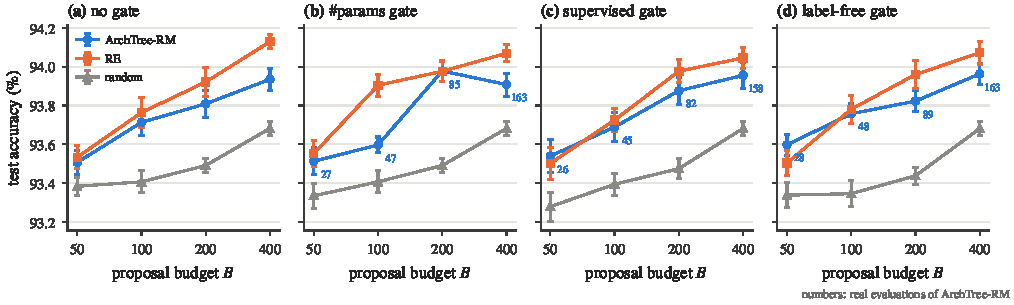
\includegraphics[width=\textwidth]{figs/figS14_nb101.pdf}
\caption{NAS-Bench-101: test accuracy (mean $\pm$ standard error) against the proposal budget for three proposers under each gate. Numbers give the real evaluations of \algname-RM.}
\label{f:nb101}
\end{figure}

%% =====================================================================
\section{LLM prior}\label{s:llm}

\textit{Prior strength.} Table~\ref{t:alpha} and Figure~\ref{f:alpha}(a,b) sweep $\alpha$. For $\alpha\ge0.2$ the runs are identical to those at $\alpha=0.2$, because the decayed weight $\alpha/\sqrt{t'}$ falls below the floor of 0.02 at the same iteration for all of them. The largest effect is $+$0.85\,pt on CIFAR-100 at 50 proposals, while ImageNet16-120 is negative in 7 of its 8 distinct ($\alpha$, $B$) cells (down to $-$0.63\,pt). Because the runs for $\alpha\ge0.2$ coincide, the 48 comparisons with $\alpha=0$ contain 24 distinct ones; none survives Holm correction (3 have $p<0.05$ before it), so the prior was left off in the headline system.

\begin{table}[tbp]
\caption{LLM prior strength: mean test accuracy for each $\alpha$ and, in brackets, the paired difference to $\alpha=0$ (pt). No difference is significant after Holm correction.}\label{t:alpha}
\centering\footnotesize
\begin{tabular}{@{}lcccccc@{}}
\toprule
\multirow{2}{*}{$\alpha$} & \multicolumn{2}{c}{CIFAR-10} & \multicolumn{2}{c}{CIFAR-100} & \multicolumn{2}{c}{ImageNet16-120}\\
\cmidrule(lr){2-3}\cmidrule(lr){4-5}\cmidrule(lr){6-7}
 & $B$ = 50 & $B$ = 100 & $B$ = 50 & $B$ = 100 & $B$ = 50 & $B$ = 100\\
\midrule
0 (off) & 94.04 & 94.19 & 72.19 & 73.02 & 45.91 & 46.45\\
0.05 & 94.21 (+0.17) & 94.36 (+0.17) & 72.93 (+0.74) & 73.21 (+0.19) & 45.77 ($-$0.15) & 46.34 ($-$0.11)\\
0.1 & 94.15 (+0.11) & 94.34 (+0.16) & 72.69 (+0.51) & 73.14 (+0.12) & 46.00 (+0.09) & 46.21 ($-$0.25)\\
0.15 & 94.25 (+0.21) & 94.27 (+0.09) & 72.96 (+0.77) & 73.20 (+0.18) & 45.69 ($-$0.22) & 45.82 ($-$0.63)\\
0.2 & 94.24 (+0.21) & 94.29 (+0.11) & 73.04 (+0.85) & 73.31 (+0.29) & 45.87 ($-$0.05) & 46.44 ($-$0.02)\\
0.3 & 94.24 (+0.21) & 94.29 (+0.11) & 73.04 (+0.85) & 73.31 (+0.29) & 45.87 ($-$0.05) & 46.44 ($-$0.02)\\
0.5 & 94.24 (+0.21) & 94.29 (+0.11) & 73.04 (+0.85) & 73.31 (+0.29) & 45.87 ($-$0.05) & 46.44 ($-$0.02)\\
0.7 & 94.24 (+0.21) & 94.29 (+0.11) & 73.04 (+0.85) & 73.31 (+0.29) & 45.87 ($-$0.05) & 46.44 ($-$0.02)\\
1 & 94.24 (+0.21) & 94.29 (+0.11) & 73.04 (+0.85) & 73.31 (+0.29) & 45.87 ($-$0.05) & 46.44 ($-$0.02)\\
\bottomrule
\end{tabular}

\end{table}

\begin{figure}[tbp]
\centering
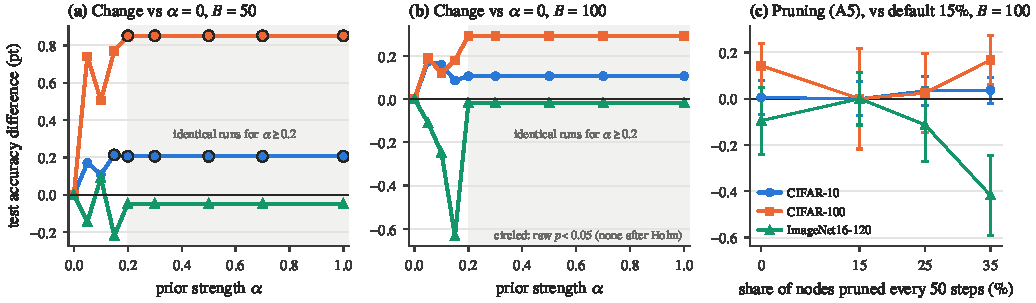
\includegraphics[width=\textwidth]{figs/figS10_alpha_prune.pdf}
\caption{(a), (b) Change in test accuracy relative to $\alpha=0$ for each prior strength at budgets 50 and 100 (circled: $p<0.05$ before correction). The shaded region gives identical runs. (c) Effect of the pruned share (A5) relative to the default of 15\% (mean $\pm$ standard error).}
\label{f:alpha}
\end{figure}

\textit{Speed of convergence.} Table~\ref{t:conv} and Figure~\ref{f:conv} measure how quickly each arm approaches the best validation accuracy in the space at $B$ = 100. On CIFAR-10 the LLM prior needs 5.0 real evaluations to come within 1\,pt (15.5 without it), and on CIFAR-100 15.6 (30.8, with one seed never getting there); on ImageNet16-120 it is slower (23.2 against 17.8). The prior with described operations is also fast on CIFAR-10 (7.8), and the size prior without any LLM matches much of the gain on CIFAR-100 (19.7) but not on ImageNet16-120. Final validation accuracies of the four arms are within 0.5\,pt of each other on every dataset.

\begin{table}[tbp]
\caption{Convergence at $B$ = 100 (means over 12 seeds): best validation accuracy after 10 and 25 real evaluations, final value, and real evaluations needed to come within 2, 1 and 0.5\,pt of the best validation accuracy in the space (seeds that never got there are counted at the end of their run; in brackets: seeds that got there, if fewer than 12).}\label{t:conv}
\centering\footnotesize
\setlength{\tabcolsep}{4pt}
\begin{tabular}{@{}llrrrrrrr@{}}
\toprule
Dataset & Arm & best@10 & best@25 & final & evals to 2\,pt & to 1\,pt & to 0.5\,pt & real evals\\
\midrule
CIFAR-10 & prior off ($\alpha$=0) & 90.38 & 91.19 & 91.47 & 5.0 & 15.5 & 22.9 & 47.8\\
 & LLM prior (standard) & 91.03 & 91.47 & 91.55 & 2.0 & 5.0 & 12.5 & 45.0\\
 & LLM prior (described ops) & 90.74 & 91.37 & 91.53 & 1.0 & 7.8 & 23.3 & 45.8\\
 & size prior (no LLM) & 90.20 & 91.52 & 91.56 & 1.0 & 16.4 & 16.4 & 37.6\\
\midrule
CIFAR-100 & prior off ($\alpha$=0) & 70.21 & 72.10 & 73.10 & 22.0 (11/12) & 30.8 (11/12) & 36.1 (8/12) & 47.1\\
 & LLM prior (standard) & 70.75 & 73.08 & 73.30 & 13.2 & 15.6 & 27.1 (9/12) & 42.8\\
 & LLM prior (described ops) & 70.81 & 72.40 & 73.20 & 21.2 & 25.4 & 35.7 (9/12) & 43.6\\
 & size prior (no LLM) & 70.83 & 73.15 & 73.43 & 17.4 & 19.7 & 20.6 & 41.0\\
\midrule
ImageNet16-120 & prior off ($\alpha$=0) & 43.75 & 45.84 & 46.42 & 14.2 & 17.8 & 24.4 (11/12) & 45.4\\
 & LLM prior (standard) & 43.90 & 45.96 & 46.49 & 14.6 & 23.2 & 32.6 (11/12) & 48.2\\
 & LLM prior (described ops) & 44.98 & 46.07 & 46.47 & 1.0 & 19.4 & 26.2 & 44.8\\
 & size prior (no LLM) & 42.80 & 45.73 & 46.08 & 15.4 & 31.2 (8/12) & 34.7 (6/12) & 46.4\\
\bottomrule
\end{tabular}

\end{table}

\begin{figure}[tbp]
\centering
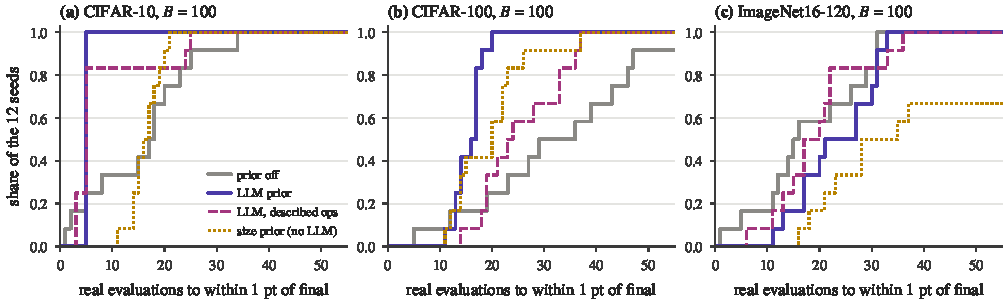
\includegraphics[width=\textwidth]{figs/figS11_convergence_ecdf.pdf}
\caption{Share of the 12 seeds that have come within 1\,pt of the best validation accuracy in the space after a given number of real evaluations ($B$ = 100). Curves that end below 1 have seeds that never got there.}
\label{f:conv}
\end{figure}

\textit{What the LLM knows.} Tables~\ref{t:probe} and~\ref{t:probetests} and Figure~\ref{f:probe} test whether the prior reflects knowledge of operations or recall of the benchmark. With operation names the LLM ranks the five operations with $\rho$ = 0.50--0.57; with the operations described but not named it does better (0.64--0.70), and with anonymous tokens it falls to 0.14--0.19, which is still above chance. A prior that simply prefers larger operations, with no LLM, scores higher than every LLM variant (0.73--0.76). The LLM therefore encodes mostly general knowledge about operation capacity, not memorised benchmark tables. Table~\ref{t:llmsize} shows that a 7B model ranks worse (0.41) and fails to answer in 3.8\% of calls, whereas the 20B and 120B models are similar in $\rho$ (0.60 and 0.61), although the larger one more often puts the best operation first (0.65 against 0.46).

\begin{table}[tbp]
\caption{LLM knowledge probe on NAS-Bench-201 (56 prefixes per dataset): mean Spearman $\rho$ between the scores given to the candidate operations and their true ranking, and share of prefixes where the top-scored operation is the best.}\label{t:probe}
\centering\footnotesize
\begin{tabular}{@{}lrrrrrr@{}}
\toprule
\multirow{2}{*}{Probe} & \multicolumn{2}{c}{CIFAR-10} & \multicolumn{2}{c}{CIFAR-100} & \multicolumn{2}{c}{ImageNet16-120}\\
\cmidrule(lr){2-3}\cmidrule(lr){4-5}\cmidrule(lr){6-7}
 & $\rho$ & top-1 & $\rho$ & top-1 & $\rho$ & top-1\\
\midrule
standard prompt (op names) & 0.57 & 0.52 & 0.50 & 0.55 & 0.52 & 0.45\\
operations described, names hidden & 0.70 & 0.57 & 0.64 & 0.52 & 0.66 & 0.54\\
anonymous tokens & 0.14 & 0.11 & 0.19 & 0.11 & 0.18 & 0.18\\
size prior (no LLM) & 0.76 & 0.80 & 0.75 & 0.86 & 0.73 & 0.73\\
\bottomrule
\end{tabular}

\end{table}

\begin{table}[tbp]
\caption{Paired tests of the probe (Wilcoxon over the 56 prefixes, Holm-corrected; difference in Spearman $\rho$).}\label{t:probetests}
\centering\footnotesize
\begin{tabular}{@{}llrrrl@{}}
\toprule
Dataset & Comparison & $n$ & mean diff. ($\rho$) & $p_{\mathrm{Holm}}$ & sig.\\
\midrule
CIFAR-10 & anonymous vs chance & 56 & 0.140 & 0.029 & yes\\
 & described vs chance & 56 & 0.701 & $<$0.001 & yes\\
 & size prior vs chance & 56 & 0.765 & $<$0.001 & yes\\
 & standard vs chance & 56 & 0.574 & $<$0.001 & yes\\
 & standard vs anonymous & 56 & 0.434 & $<$0.001 & yes\\
 & standard vs described & 56 & $-$0.127 & 0.002 & yes\\
 & standard vs size prior & 56 & $-$0.191 & 0.001 & yes\\
\midrule
CIFAR-100 & anonymous vs chance & 56 & 0.190 & 0.007 & yes\\
 & described vs chance & 56 & 0.640 & $<$0.001 & yes\\
 & size prior vs chance & 56 & 0.751 & $<$0.001 & yes\\
 & standard vs chance & 56 & 0.500 & $<$0.001 & yes\\
 & standard vs anonymous & 56 & 0.310 & $<$0.001 & yes\\
 & standard vs described & 56 & $-$0.141 & 0.001 & yes\\
 & standard vs size prior & 56 & $-$0.251 & $<$0.001 & yes\\
\midrule
ImageNet16-120 & anonymous vs chance & 56 & 0.181 & 0.007 & yes\\
 & described vs chance & 56 & 0.661 & $<$0.001 & yes\\
 & size prior vs chance & 56 & 0.733 & $<$0.001 & yes\\
 & standard vs chance & 56 & 0.516 & $<$0.001 & yes\\
 & standard vs anonymous & 56 & 0.334 & $<$0.001 & yes\\
 & standard vs described & 56 & $-$0.145 & $<$0.001 & yes\\
 & standard vs size prior & 56 & $-$0.217 & $<$0.001 & yes\\
\bottomrule
\end{tabular}

\end{table}

\begin{table}[tbp]
\caption{Model size (CIFAR-10, 26 prefixes): mean Spearman $\rho$, top-1 hit rate, share of calls that fell back to uniform scores and operation-name errors per call.}\label{t:llmsize}
\centering\footnotesize
\begin{tabular}{@{}lrrrrr@{}}
\toprule
Model & prefixes & mean $\rho$ & top-1 hit & fallback (\%) & op-name errors / call\\
\midrule
\texttt{allam-2-7b} & 26 & 0.41 & 0.50 & 3.8 & 0.50\\
\texttt{openai/gpt-oss-120b} & 26 & 0.61 & 0.65 & 0.0 & 0.00\\
\texttt{openai/gpt-oss-20b} & 26 & 0.60 & 0.46 & 0.0 & 0.00\\
\bottomrule
\end{tabular}

\end{table}

\begin{figure}[tbp]
\centering
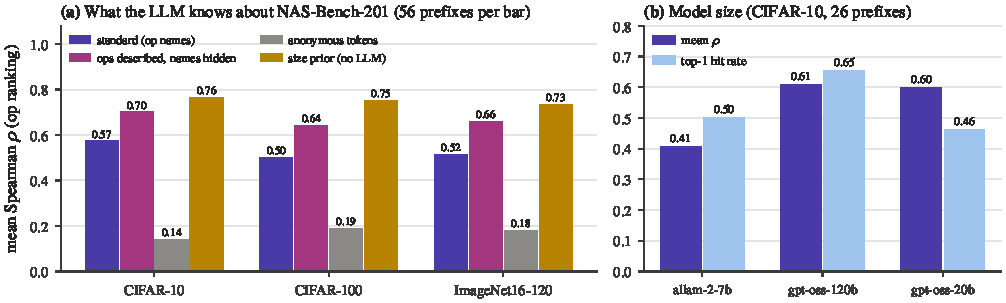
\includegraphics[width=\textwidth]{figs/figS12_llm_probes.pdf}
\caption{(a) Mean Spearman correlation between LLM scores and the true ranking of operations under four prompt conditions. (b) The same for three model sizes on CIFAR-10.}
\label{f:probe}
\end{figure}

%% =====================================================================
\section{Hardware-aware search}\label{s:hw}

Table~\ref{t:hw} gives hypervolume (relative to random search), inverted generational distance (IGD) and front size for every device and budget, and Figure~\ref{f:hw} the IGD and front-size curves. The hypervolumes of \algname-HW and NSGA-II-style search lie within 0.5\% of random search everywhere (99.89--100.42\%), and all 96 tests are ties after Holm correction (22 have $p<0.05$ before it, mostly small hypervolume gains of \algname-HW): on HW-NAS-Bench the accuracy--latency front is easy to cover, and no difference between the methods survives correction. IGD separates them somewhat more: at 25 proposals \algname-HW is the furthest from the true front on all six devices, and NSGA-II-style search finds the largest fronts in 18 of 24 device--budget cells (Figure~\ref{f:hw}b); at 200 proposals the differences are small, NSGA-II-style search having the lowest IGD on four of the six devices.

\begin{table}[tbp]
\caption{HW-NAS-Bench (CIFAR-10): hypervolume as \% of random search, IGD to the true front, and mean size of the front found by \algname-HW (12 seeds).}\label{t:hw}
\centering\footnotesize
\begin{tabular}{@{}lrrrrrrr@{}}
\toprule
\multirow{2}{*}{Device} & \multirow{2}{*}{$B$} & \multicolumn{2}{c}{HV (\% of random)} & \multicolumn{3}{c}{IGD} & front\\
\cmidrule(lr){3-4}\cmidrule(lr){5-7}
 & & ArchTree-HW & NSGA-II-style & ArchTree-HW & NSGA-II-style & random & size\\
\midrule
Edge GPU & 25 & 100.04 & 99.96 & 23.31 & 14.22 & 13.67 & 5.2\\
 & 50 & 100.38 & 100.15 & 15.98 & 9.94 & 9.81 & 6.4\\
 & 100 & 100.39 & 100.09 & 7.03 & 2.52 & 7.21 & 9.7\\
 & 200 & 100.32 & 100.13 & 0.22 & 0.17 & 0.38 & 12.6\\
\midrule
Raspberry Pi 4 & 25 & 99.89 & 99.95 & 11.07 & 9.24 & 8.08 & 6.6\\
 & 50 & 100.23 & 100.07 & 7.73 & 8.04 & 5.90 & 10.1\\
 & 100 & 100.05 & 100.19 & 2.60 & 4.06 & 4.35 & 12.9\\
 & 200 & 100.14 & 100.31 & 2.04 & 1.78 & 1.31 & 18.4\\
\midrule
Edge TPU & 25 & 100.01 & 99.94 & 1.35 & 1.16 & 1.04 & 3.8\\
 & 50 & 100.42 & 100.24 & 0.65 & 0.80 & 0.76 & 7.9\\
 & 100 & 100.23 & 100.15 & 0.34 & 0.48 & 0.50 & 10.8\\
 & 200 & 100.24 & 100.27 & 0.22 & 0.15 & 0.26 & 13.3\\
\midrule
Pixel 3 & 25 & 100.08 & 99.96 & 9.36 & 7.98 & 6.92 & 7.0\\
 & 50 & 100.18 & 100.02 & 7.71 & 7.41 & 4.97 & 9.4\\
 & 100 & 100.27 & 100.06 & 4.40 & 6.12 & 3.73 & 12.6\\
 & 200 & 100.21 & 100.22 & 0.69 & 1.44 & 0.80 & 18.0\\
\midrule
Eyeriss & 25 & 100.16 & 99.94 & 1.54 & 1.28 & 1.24 & 3.8\\
 & 50 & 100.35 & 100.09 & 1.17 & 0.99 & 1.07 & 6.5\\
 & 100 & 100.32 & 100.25 & 0.78 & 0.58 & 0.81 & 8.7\\
 & 200 & 100.34 & 100.26 & 0.51 & 0.34 & 0.64 & 11.0\\
\midrule
FPGA & 25 & 100.25 & 99.96 & 1.33 & 1.15 & 1.15 & 5.8\\
 & 50 & 100.37 & 99.98 & 1.06 & 0.95 & 1.02 & 7.4\\
 & 100 & 100.36 & 100.08 & 0.78 & 0.60 & 0.82 & 8.7\\
 & 200 & 100.37 & 100.26 & 0.55 & 0.35 & 0.64 & 11.1\\
\bottomrule
\end{tabular}

\end{table}

\begin{figure}[tbp]
\centering
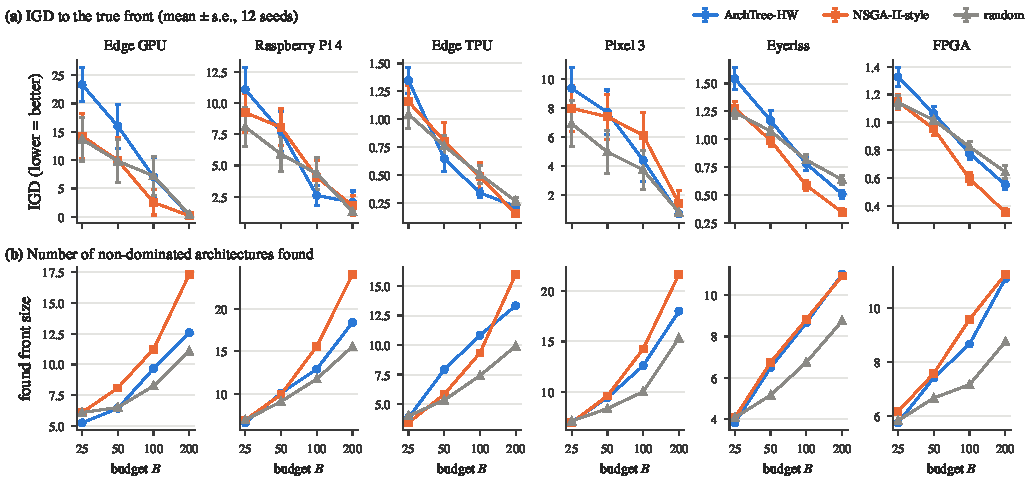
\includegraphics[width=\textwidth]{figs/figS13_hw_igd.pdf}
\caption{Hardware-aware search on the six HW-NAS-Bench devices. (a) IGD between the found and the true accuracy--latency front (mean $\pm$ standard error). (b) Number of non-dominated architectures found.}
\label{f:hw}
\end{figure}

Table~\ref{t:crossdev} compares the true fronts of the devices. Few architectures are shared (Jaccard 0.06--0.40) although latencies are correlated ($\rho$ = 0.51--0.97). Yet a front computed for one device, when evaluated on another, keeps 83--100\% of the hypervolume of that device's true front. Fronts differ in membership far more than in quality, so a search for one device is a reasonable starting point for another, while the exact Pareto set must be searched per device.

\begin{table}[tbp]
\caption{True Pareto fronts of each device pair (CIFAR-10): front sizes, shared architectures, Jaccard index, Spearman correlation of latency over all architectures, and hypervolume ratio when the front of one device is used on the other.}\label{t:crossdev}
\centering\footnotesize
\begin{tabular}{@{}lrrrrrr@{}}
\toprule
Device pair ($a$ -- $b$) & front sizes & shared & Jaccard & $\rho$(latency) & HV ratio $a\to b$ & HV ratio $b\to a$\\
\midrule
Edge GPU -- Raspberry Pi 4 & 24 / 48 & 6 & 0.09 & 0.65 & 0.992 & 0.998\\
Edge GPU -- Edge TPU & 24 / 43 & 4 & 0.06 & 0.70 & 0.991 & 0.989\\
Edge GPU -- Pixel 3 & 24 / 55 & 5 & 0.07 & 0.63 & 0.988 & 0.997\\
Edge GPU -- Eyeriss & 24 / 17 & 3 & 0.08 & 0.51 & 0.969 & 0.833\\
Edge GPU -- FPGA & 24 / 11 & 4 & 0.13 & 0.62 & 0.950 & 0.833\\
Raspberry Pi 4 -- Edge TPU & 48 / 43 & 9 & 0.11 & 0.59 & 0.996 & 0.995\\
Raspberry Pi 4 -- Pixel 3 & 48 / 55 & 13 & 0.14 & 0.97 & 0.999 & 0.998\\
Raspberry Pi 4 -- Eyeriss & 48 / 17 & 7 & 0.12 & 0.68 & 1.000 & 0.994\\
Raspberry Pi 4 -- FPGA & 48 / 11 & 7 & 0.13 & 0.89 & 1.000 & 0.994\\
Edge TPU -- Pixel 3 & 43 / 55 & 8 & 0.09 & 0.63 & 0.987 & 0.996\\
Edge TPU -- Eyeriss & 43 / 17 & 6 & 0.11 & 0.82 & 0.995 & 0.988\\
Edge TPU -- FPGA & 43 / 11 & 7 & 0.15 & 0.53 & 0.998 & 0.988\\
Pixel 3 -- Eyeriss & 55 / 17 & 9 & 0.14 & 0.72 & 0.999 & 0.986\\
Pixel 3 -- FPGA & 55 / 11 & 7 & 0.12 & 0.87 & 0.998 & 0.985\\
Eyeriss -- FPGA & 17 / 11 & 8 & 0.40 & 0.75 & 1.000 & 0.999\\
\bottomrule
\end{tabular}

\end{table}

%% =====================================================================
\section{Seeds, reproducibility checks and data}\label{s:repro}

Table~\ref{t:checks} lists the reproducibility checks, Table~\ref{t:checksums} the SHA-256 checksums of the data, Table~\ref{t:datastore} the derived files the experiments read and Table~\ref{t:env} the software environment.

\textit{Seeds.} Main seeds (all experiments): 42, 111, 123, 222, 333, 456, 789, 999, 1001, 2024, 31415, 27182. Held-out seeds (design ablation only, never used for a design decision): 7, 13, 77, 101, 202, 303, 404, 505, 606, 707, 808, 909. Proxy calibration draws its 1,500 architectures with seed 0, and the proxy network is initialised with seed 1234. Every run seeds its own random number generators, so results do not depend on the order or the number of parallel workers.

\begin{table}[tbp]
\caption{Reproducibility checks carried out on the final code.}\label{t:checks}
\centering\footnotesize
\begin{tabular}{@{}>{\raggedright\arraybackslash}p{0.42\textwidth}>{\raggedright\arraybackslash}p{0.52\textwidth}@{}}
\toprule
Check & Result\\
\midrule
Parallel workers (equal GPU-hours) & 1 and 3 workers give identical results (252 of 252 runs)\\
Device rerun against the offline replica & identical (Phase 3: 108 of 108 runs; design ablation: 540 of 540)\\
A1, A3, A6 against the headline runs & identical (144 of 144 runs each; Table~\ref{t:toggles})\\
Zero-information LLM prior against $\alpha=0$ & identical on 24 of 24 seeds\\
Repeated real evaluations in \algname{} runs & 0 in every run (Table~\ref{t:dups})\\
NAS-Bench-201 path after the NB101 refactor & bit-identical (6 of 6 regression runs)\\
TensorFlow-free NAS-Bench-101 reader & all 423,624 graph hashes reproduced\\
Shared proxy cache under a file lock & no entry lost with 4 concurrent workers\\
HW-NAS-Bench architecture alignment & accuracy--latency Spearman $\rho$ = 0.624 after re-indexing\\
Equal-GPU-hour runs below budget & 5 of 1,128 (proposals exhausted at $k=100$; section~\ref{s:egh})\\
LLM fallbacks & 0 in LLM-prior runs; 0.37 random replacements per LLM-NAS run\\
\bottomrule
\end{tabular}
\end{table}

\begin{table}[tbp]
\caption{Data files used for the paper (SHA-256).}\label{t:checksums}
\centering\scriptsize
\begin{tabular}{@{}lr>{\ttfamily}l@{}}
\toprule
File & Size (bytes) & \normalfont SHA-256\\
\midrule
NAS-Bench-201-v1\_1-096897.pth & 5,003,180,601 & 2317a7dc911654322f4f932730a821cf38ecc5b5f1adde0aff26ff6b3f736666\\
nasbench\_only108.tfrecord & 522,767,376 & 4c39c3936e36a85269881d659e44e61a245babcb72cb374eacacf75d0e5f4fd1\\
nb201\_cache\_v2.json & 4,894,199 & b6f19d2d0adee7b09d3a9ff098a379695d3c224cdcf5dafeb25f0924afee2694\\
nb101\_cache.npz & 22,126,761 & 4e0fb9901ff6952fc1d345c6ee1be8f6c7b4406c0f0843bbd255bc14a302d19e\\
natssss\_cache.json & 12,828,328 & 8cac2574ab56b07dcf9b82461e03d0195a34a0187eb4239b362f940cdd28d18a\\
HW-NAS-Bench-v1\_0.pickle & 10,782,467 & 57f92c2d7b88814fa337d00f4597c8ca30d507c5a855c18d6fac57e5ad872700\\
\bottomrule
\end{tabular}
\end{table}

\begin{table}[tbp]
\caption{Derived data files read by the experiments (moved from the main paper).}\label{t:datastore}
\centering\footnotesize
\setlength{\tabcolsep}{2pt}
\begin{tabular}{@{}>{\raggedright\arraybackslash}p{0.22\textwidth}>{\raggedright\arraybackslash}p{0.18\textwidth}>{\raggedright\arraybackslash}p{0.42\textwidth}>{\raggedleft\arraybackslash}p{0.1\textwidth}@{}}
\toprule
File & Key & Fields per architecture & Size\\
\midrule
NB201 cache (JSON) & base-5 index & valid, test, train time $\times$ 3 datasets & 4.9\,MB\\
NB101 cache (NPZ) & module hash & adjacency, ops, \#params, valid/test/time $\times$ 3 repeats & 22\,MB\\
NATS-SSS cache (JSON) & base-8 code & valid, test, train time $\times$ 3 datasets; \#params, FLOPs & 12.8\,MB\\
HW table (NPZ) & NB201 index & accuracy, latency on 6 devices & 0.9\,MB\\
True fronts (JSON) & device & Pareto-optimal (accuracy, latency) pairs & $<$3\,kB\\
Proxy cache (JSON) & token string & raw $E$, $S$, $T$, size term & 12\,MB\\
\bottomrule
\end{tabular}
\tablenotes{Search uses the validation split; test accuracy is only reported. C10 validation in NB201 is the \texttt{cifar10-valid} split, as prescribed by the benchmark.}
\end{table}

\begin{table}[tbp]
\caption{Software and hardware environment of the runs.}\label{t:env}
\centering\footnotesize
\begin{tabular}{@{}ll@{\hspace{2.5em}}ll@{}}
\toprule
Item & Version & Item & Version\\
\midrule
Python & 3.10.9 & PyTorch / torchvision & 2.5.1 / 0.20.1 (CUDA 12.4)\\
NumPy & 2.2.6 & SciPy & 1.15.3\\
pandas & 2.3.3 & Matplotlib & 3.10.9\\
nas-bench-201 & 2.1 & groq client & 1.5.0\\
GPU & NVIDIA GeForce RTX 2050, 4\,GB & OS & Windows 11 (build 26300)\\
\bottomrule
\end{tabular}
\tn{The complete pinned package list is \texttt{outputs/final/repro/requirements.lock.txt} in the repository. Tabular look-ups are deterministic; the proxy kernels use cuDNN benchmark mode, so raw proxy scores are cached and shipped with the code to make them identical across machines. LLM answers are cached per prompt and shipped for exact replay.}
\end{table}

{\sloppy\textit{Run order.} The results are regenerated by building the benchmark caches (\texttt{tools/build\_nb201\_cache.py}, \texttt{tools/build\_nb101\_cache.py}), running the experiments in the order of Table~2 of the main paper (\texttt{experiments/run\_phase0.py} to \texttt{run\_equal\_gpu\_hours.py}), aggregating the statistics (\texttt{run\_phase6\_aggregate.py}) and finally running \texttt{make\_figures.py} and the two supplementary scripts. The PowerShell script \texttt{run\_full\_pipeline.ps1} in the repository performs all steps in sequence.\par}

%% =====================================================================
\begin{thebibliography}{99}
\bibitem{kocsis2006} Kocsis L and Szepesv\'{a}ri C 2006 Bandit based Monte-Carlo planning. In: \textit{Proceedings of the European Conference on Machine Learning}, LNCS 4212, pp. 282--293
\bibitem{coquelin2007} Coquelin P A and Munos R 2007 Bandit algorithms for tree search. In: \textit{Proceedings of the 23rd Conference on Uncertainty in Artificial Intelligence}, pp. 67--74
\bibitem{bubeck2011} Bubeck S, Munos R, Stoltz G and Szepesv\'{a}ri C 2011 X-armed bandits. \textit{J. Mach. Learn. Res.} 12: 1655--1695
\end{thebibliography}

\end{document}
